\chapter{Ionization yield}\label{chap:18}
A deposit of \SI{10}{eV} in silicon has enough energy for eight electron--hole pairs across the \SI{1.17}{eV} gap of silicon at millikelvin temperatures, yet the cascade model of \cref{sec:18.1} leaves two or three in nearly every event. The measured mean energy per pair is three times the gap (\cref{sec:18.4}), and the rest of the energy ends in phonons. Between the deposit and the count lies a cascade of hot carriers that ionize, emit phonons and slow down, all within about a picosecond. The mean energy per pair $\varepsilon_{\mathrm{eh}}$ and the Fano factor $F_{\mathrm{eh}}$ of the pair number set the threshold of every electron-recoil search in a semiconductor, since at the few-pair level one ionization more or less moves an event from one bin to the next. For a long time both have been fitted to calibration data rather than computed: the cascade model used for silicon has one constant, tuned to the measured $\varepsilon_{\mathrm{eh}}$ (\cref{app:E.13}).

This chapter asks how far the two numbers can be derived from the rates of the master formula. The hot carrier is itself a projectile of the master formula. It scatters off the electrons and the lattice of the target as a dark-matter particle with a Coulomb coupling would, which \cref{sec:4.8} already found for the quasiparticle lifetime of an electron gas. The cascade also inherits the split of energy between the electron and the hole that the dark-matter interaction made. A pair made at a momentum transfer of a few keV shares its energy between electron and hole differently from a pair made by a photon (\cref{sec:8.7}), and at a few pairs that difference can be a whole ionization. The chapters that follow take the deposit to the quanta a sensor counts, then to a limit and to a guide to the next targets (\cref{fig:18-map}).

\begin{figure}[tbp]
  \centering
  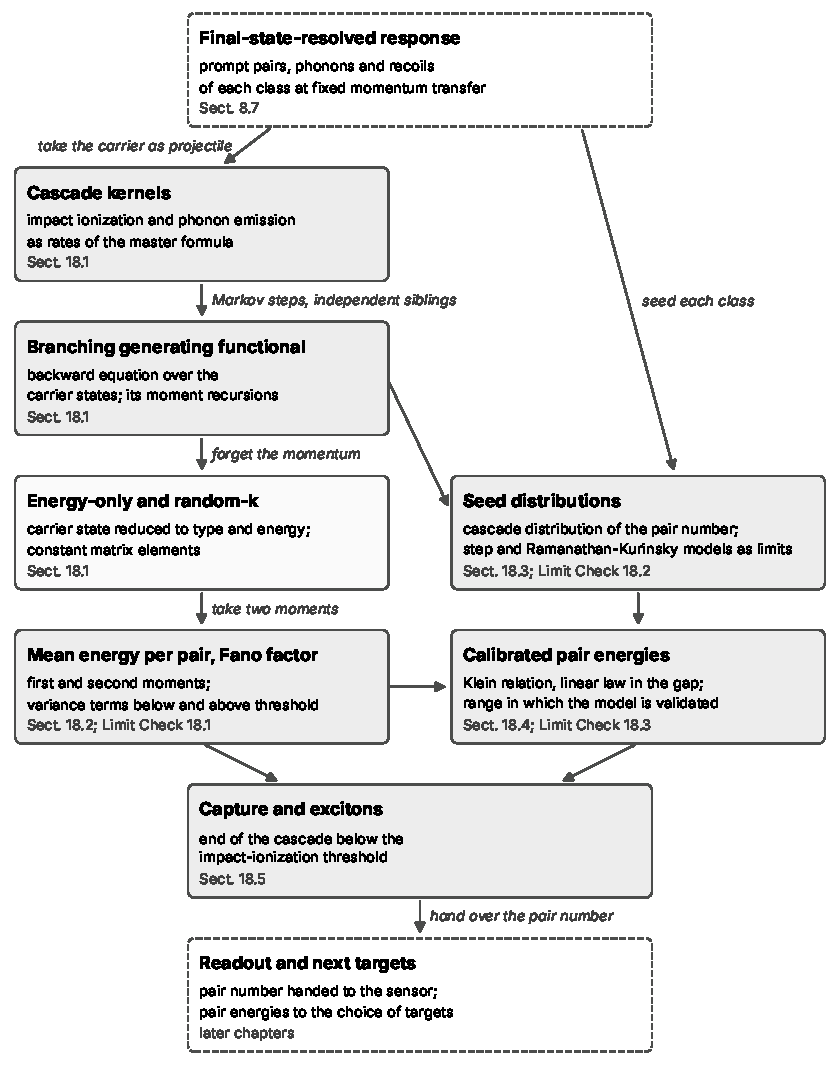
\includegraphics[width=0.85\linewidth]{figures/ch18/map18.pdf}
  \caption{Ionization yield, from the final-state-resolved response of \cref{sec:8.7} to the pair number. Main line: impact ionization and phonon emission as rates of the master formula with the carrier as projectile, the branching generating functional of the cascade and its reduction to carrier energies alone (\cref{sec:18.1}), then the mean energy per pair and the Fano factor as its first two moments (\cref{sec:18.2}; \cref{lim:18.2a,lim:18.2b}). Side branches: the seeding of the cascade by each final-state class, with the step model and the Ramanathan--Kurinsky model as its limits (\cref{sec:18.3}; \cref{lim:18.3a}), and the calibrated pair energies of silicon, germanium, GaAs and the wide-gap crystals with the range in which the cascade model is validated (\cref{sec:18.4}; \cref{lim:18.4a,lim:18.4c}). Both feed the end of the cascade below the impact-ionization threshold, capture and excitons (\cref{sec:18.5}), which hands the pair number to the readout and the pair energies to the choice of new targets.}
  \label{fig:18-map}
\end{figure}

\section{The carrier cascade}\label{sec:18.1}

In the cascade model of silicon built in this section, an electron with \SI{50}{eV} of kinetic energy makes about 13 new electron--hole pairs before every carrier has fallen below the threshold for impact ionization, and the remaining \SI{35}{eV} goes to the lattice. \Cref{fig:18-tree} shows one such cascade. Each step in the cascade is a collision of a hot carrier with the target: either the carrier lifts a valence electron across the gap, or it emits a phonon. Impact ionization and phonon emission are both scattering events of a projectile off the electrons or the nuclei of the crystal, and each is a rate of the master formula \cref{eq:8.2-rate} with the carrier in the place of the dark-matter particle. The cascade is then a branching process whose kernels are those rates, and its statistics follow from one generating functional that obeys a recursion in energy. Two reductions make the recursion solvable: the energy-only reduction drops the momentum of each carrier, and the random-$k$ reduction also replaces the matrix elements by constants. The electron and the hole that the dark matter leaves behind form the seed of the cascade. Both reductions must keep the seed, because at a few pairs the way the two seed carriers share the energy changes the count.

\begin{figure}[tbp]
  \centering
  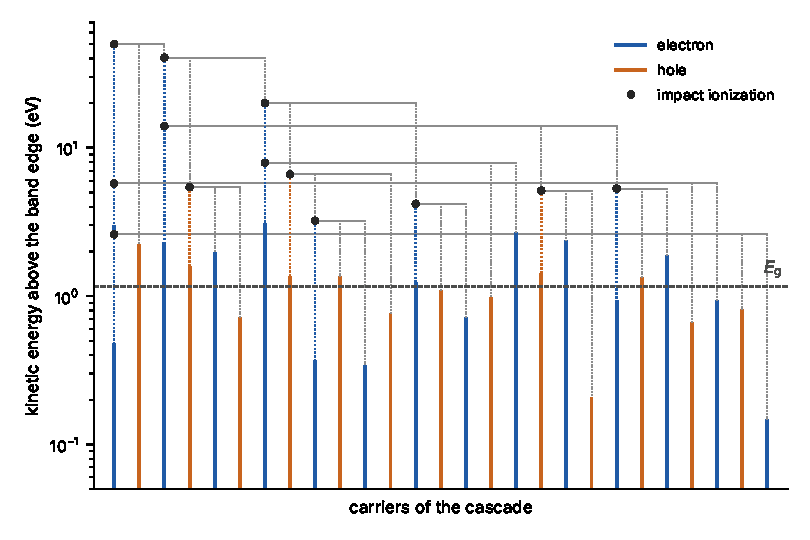
\includegraphics[width=0.95\linewidth]{figures/ch18/fig18_1.pdf}
  \caption{One sampled cascade started by an electron with \SI{50}{eV} of kinetic energy in silicon, in the energy-only random-$k$ model of \cref{sec:18.1-reductions}: free-particle densities of states, constant matrix elements, impact ionization above $\Eg = \SI{1.160}{eV}$ (silicon at \SI{123}{K}; threshold ratio $\theta_{\mathrm{ii}} = 1$), one optical phonon of \SI{63}{meV}, the rate ratio \cref{eq:18.1-randomk} with $A_{\mathrm{AB}} = \SI{5.703}{eV^3}$ (calibrated in \cref{sec:18.4}), and holes confined to the \SI{12}{eV} valence band. Each column is one carrier (blue electrons, orange holes), drawn from the kinetic energy at which it was created down to the band edge, on a logarithmic axis. Solid segments are runs of phonon emission; a dot marks an impact ionization, after which the carrier continues at the lower energy reached along the dotted segment, and the grey lines lead to the two carriers created in the ionization. This cascade has 13 ionizations, 27 carriers and 176 phonon emissions, every emission made by a carrier below \SI{6}{eV}, and leaves \SI{34.9}{eV} as heat. On average the model makes 12.99 new pairs, \SI{3.85}{eV} per pair at this energy, with a variance of 0.119 times the mean (generating function of \cref{sec:18.3}).}
  \label{fig:18-tree}
\end{figure}

\subsection{Impact ionization as a master-formula rate}\label{sec:18.1-ii}

A carrier in the Bloch state $n\vect{k}$, an electron in a conduction band or a hole in a valence band, interacts with every other charge of the crystal through the Coulomb potential. It is charged, so it couples to the total charge density $n_Z$ of electrons and nuclei, as a dark photon does (\cref{sec:8.4}). In a collision it gives a momentum $\vect{p}$ to the target and ends in a state $n'$, $\vect{k} - \vect{p}$; we write $\vect{p}$ for the momentum transfer of the carrier and keep $\vect{q}$ for the dark-matter momentum transfer that made the seed. Because the carrier is a Bloch wave and not a plane wave, the momenta $\vect{p} + \vect{G}$ for all reciprocal-lattice vectors $\vect{G}$ lead to the same final carrier state, and their amplitudes add. With $\vect{p}$ in the first zone, the amplitude to reach $n'$, $\vect{k} - \vect{p}$ and the target state $|f\rangle$ is
\begin{equation*}
  \frac{1}{\Vol}\sum_{\vect{G}}v_{\mathrm{C}}(|\vect{p}+\vect{G}|)\,\rho_{n'n}(\vect{k},-\vect{p}-\vect{G})\,\langle f|n_Z(\vect{p}+\vect{G})|i\rangle ,
\end{equation*}
with the overlap $\rho_{n'n}$ of \cref{eq:3.2-rho} in the place of the plane-wave overlap of a free projectile. This amplitude comes from the interaction \cref{eq:8.1-Hint} with one coupling row for each $\vect{G}$, the potential $\tilde V_{\vect{G}} = v_{\mathrm{C}}(|\vect{p}+\vect{G}|)\,\rho_{n'n}(\vect{k},-\vect{p}-\vect{G})$, and the target operators $n_Z(\vect{p}+\vect{G})$. The master formula \cref{eq:8.2-rate} then yields the rate directly, with two changes. The sum over final projectile states runs over the bands $n'$ and the first zone instead of over all momenta. And the final carrier state must be empty, which adds the factor $1 - f_{n',\vect{k}-\vect{p}}$. The response matrix that appears is $S_{\vect{G}\vect{G}'}(\vect{p},\omega)$ of the total charge, at the energy $\omega = \varepsilon_{n\vect{k}} - \varepsilon_{n',\vect{k}-\vect{p}}$ that the carrier loses.

The fluctuation--dissipation theorem turns this response into the screened interaction. With $R$ the retarded density response of \cref{sec:8.7}, at $\omega > 0$ the theorem reads $S = -2\,(1 + n_{\mathrm{B}}(\omega))\,(R - R^\dagger)/2\ii$ as a matrix in $\vect{G}$, the matrix form of the relation used in \cref{sec:8.7}, with $1/(1 - \ee^{-\beta\omega}) = 1 + n_{\mathrm{B}}(\omega)$. Sandwiched between Coulomb kernels, $R$ gives $v_{\mathrm{C}}Rv_{\mathrm{C}} = W^{\mathrm{scr}} - v_{\mathrm{C}}$ by \cref{eq:4.8-W}, and the bare $v_{\mathrm{C}}$ is real and diagonal and drops out of the anti-Hermitian part of $v_{\mathrm{C}}Rv_{\mathrm{C}}$. With the dielectric matrix of electrons and nuclei together in $W^{\mathrm{scr}}$:
\begin{keyresult}[Impact-ionization kernel]
\begin{equation}
  \varGamma_{\mathrm{ii}}(n\vect{k}) = -2\sum_{n'}\int_{\mathrm{BZ}}\frac{\dd^3p}{(2\pi)^3}\sum_{\vect{G}\vect{G}'}\rho_{\vect{G}}^*\,\Bigl[\frac{W^{\mathrm{scr}} - W^{\mathrm{scr}\dagger}}{2\ii}\Bigr]_{\vect{G}\vect{G}'}\!(\vect{p},\omega)\;\rho_{\vect{G}'}\;\bigl[1 - f_{n',\vect{k}-\vect{p}}\bigr]\bigl[1 + n_{\mathrm{B}}(\omega)\bigr] ,
  \label{eq:18.1-ii}
\end{equation}
with $\rho_{\vect{G}} = \rho_{n'n}(\vect{k},-\vect{p}-\vect{G})$ and $\omega = \varepsilon_{n\vect{k}} - \varepsilon_{n',\vect{k}-\vect{p}}$. Without the off-diagonal elements $\vect{G} \neq \vect{G}'$ the sum over $\vect{G}$ and the integral over the zone combine into one integral over all $\vect{p}$,
\begin{equation}
  \varGamma_{\mathrm{ii}}(n\vect{k}) \simeq \sum_{n'}\int\frac{\dd^3p}{(2\pi)^3}\,2v_{\mathrm{C}}(p)\,\bigl|\rho_{n'n}(\vect{k},-\vect{p})\bigr|^2\,L(\vect{p},\omega)\,\bigl[1 - f_{n',\vect{k}-\vect{p}}\bigr]\bigl[1 + n_{\mathrm{B}}(\omega)\bigr] ,
  \label{eq:18.1-iidiag}
\end{equation}
with $L$ the loss function \cref{eq:4.4-SL} of the total dielectric matrix at the unreduced momentum $\vect{p}$.
\end{keyresult}
\noindent For a hole the occupations are those of holes, $1 - f \to f$ in the valence bands. For a free-electron gas, $\rho = 1$ and \cref{eq:18.1-iidiag} is the out-scattering part of the lifetime \cref{eq:4.8-lifetime}: the step from \cref{sec:4.8} to here is the step from plane waves to Bloch waves and from the electron gas to a crystal with nuclei. The two terms of \cref{eq:18.1-ii} with $\vect{G} \neq \vect{G}'$ are local fields, and the master formula delivers them in their anti-Hermitian combination, which is real for any $W^{\mathrm{scr}}$, since $(W^{\mathrm{scr}} - W^{\mathrm{scr}\dagger})/2\ii$ is a Hermitian matrix and $\rho^\dagger A\rho$ is real for every Hermitian $A$. The element-wise imaginary part of $W^{\mathrm{scr}}_{\vect{G}\vect{G}'}$ agrees with the anti-Hermitian combination only when $W^{\mathrm{scr}}_{\vect{G}\vect{G}'} = W^{\mathrm{scr}}_{\vect{G}'\vect{G}}$, which holds in silicon and germanium with the origin at an inversion center but not in GaAs. The same symmetry condition separated the retarded and advanced pair weights of \cref{sec:8.7}.

The kernel is the rate at which the carrier scatters out of $n\vect{k}$. The quasiparticle width of the carrier differs from this out-scattering rate in two ways. By the cutting rule of \cref{sec:4.8}, $-2\Imag\Sigma^{\mathrm{R}} = \varGamma_{\mathrm{out}} + \varGamma_{\mathrm{in}}$. The in-scattering term carries the product $f\,n_{\mathrm{B}}$ of an occupied final state and a thermal excitation of energy $\omega \ge \Eg$, and so vanishes for a hot carrier at $T \ll \Eg$. The width also carries the quasiparticle residue, $\varGamma_{\mathrm{qp}} = -2z_{\mathrm{qp}}\Imag\Sigma^{\mathrm{R}}$ by \cref{eq:4.7-qp}, with $z_{\mathrm{qp}} \approx 0.8$ for the hot carriers of semiconductors~\cite[Sect.~II]{kotani2010impact}. \Cref{eq:18.1-ii} is first order in $W^{\mathrm{scr}}$ and sets $z_{\mathrm{qp}} = 1$. Since the factor $z_{\mathrm{qp}}$ lowers every impact-ionization rate by a nearly uniform 20 percent, a calibrated model absorbs it. The exchange of the carrier with the electron it excites is a vertex correction, absent from \cref{eq:18.1-ii} as it was from \cref{eq:4.8-lifetime}; it enters only beyond first order in $W^{\mathrm{scr}}$, and \cref{sec:18.5} lists it among the open problems.

The plasmon is inside the kernel. In silicon $\varepsilon_2$ is still 0.224 at the plasmon energy, where $\varepsilon_1$ vanishes (\cref{we:4-siplasmon}), so the plasmon peak carries the weight of electron--hole pairs. A carrier that ``emits a plasmon'' and the plasmon that ``decays into a pair'' are one term of \cref{eq:18.1-ii}, and a cascade built on \cref{eq:18.1-ii} must not add a separate plasmon channel. The plasmon becomes a particle of the cascade only where its pole is undamped and carries no pair weight, as in aluminum below the critical momentum $q_{\mathrm{c}}$ of \cref{sec:4.5}; it then needs a decay kernel of its own.

The loss function vanishes for $\omega < \Eg$ at $T \ll \Eg$, so a carrier must give up at least the gap. Energy conservation alone would let it ionize as soon as its kinetic energy $x$ above the band edge exceeds $\Eg$, but the three final carriers must also carry its crystal momentum. Take parabolic bands with an electron mass $m^*_{\mathrm{e}}$ and a hole mass $m^*_{\mathrm{h}}$. At the threshold energy, which is the lowest energy at which an electron can make a pair, the three products of the ionization move with a common velocity $\vect{u}$, so that no energy is spent on motion in their center-of-mass frame. Momentum conservation gives $m^*_{\mathrm{e}}\vect{v}_0 = (2m^*_{\mathrm{e}} + m^*_{\mathrm{h}})\vect{u}$ for an initial velocity $\vect{v}_0$, energy conservation $\tfrac12m^*_{\mathrm{e}}v_0^2 = \Eg + \tfrac12(2m^*_{\mathrm{e}} + m^*_{\mathrm{h}})u^2$, and eliminating $\vect{u}$ yields
\begin{equation}
  x_{\mathrm{th}} = \theta_{\mathrm{ii}}\Eg , \qquad \theta_{\mathrm{ii}} = \frac{2m^*_{\mathrm{e}} + m^*_{\mathrm{h}}}{m^*_{\mathrm{e}} + m^*_{\mathrm{h}}} ,
  \label{eq:18.1-theta}
\end{equation}
with $\theta_{\mathrm{ii}}$ the impact-ionization threshold ratio. Equal masses give $\theta_{\mathrm{ii}} = 3/2$; for a hole the two masses exchange places. In a real band structure the threshold is soft rather than sharp, because a crystal conserves momentum only up to $\vect{G}$ and the bands are not parabolic. Just above threshold few final states satisfy both conservation laws, and the computed rate scatters by large factors from one $\vect{k}$ to the next~\cite[Fig.~2]{kotani2010impact}.

\subsection{The phonon-emission kernel}\label{sec:18.1-ph}

The carrier also couples to the displacements of the nuclei, through the vertex $g_{mn\nu}(\vect{k},\vect{Q})$ of \cref{eq:6.2-g}. Take the phonon coordinate of branch $\nu$ at $\vect{Q}$ as the target operator and $g$ as the potential. The response of a harmonic phonon coordinate is $2\pi[(n_{\vect{Q}\nu} + 1)\delta(\omega - \omega_{\vect{Q}\nu}) + n_{\vect{Q}\nu}\delta(\omega + \omega_{\vect{Q}\nu})]$, and the master formula with the Pauli factor of the final carrier gives the out-scattering part of \cref{eq:6.3-ImFM}, the phonon kernel $\varGamma_{\mathrm{ph}}(n\vect{k})$ of \cref{eq:E.13-gph}. At detector temperatures only the emission term survives. The vertex is screened statically, as density-functional perturbation theory computes it, and the corrections to static screening are of higher order in $\omega_{\vect{Q}\nu}/\Eg$ (\cref{sec:6.2}).

In a polar crystal the two kernels overlap. The total dielectric matrix in $W^{\mathrm{scr}}$ contains the ionic response, and at $\omega$ near the longitudinal optical frequency $\omega_L$ its loss function has the Fr\"ohlich line: \cref{eq:18.1-ii} already contains the emission of a longitudinal optical phonon through the macroscopic field. The long-range vertex $g^L = \ii C_{\mathrm{F}}\rho_{mn}/Q$ of \cref{eq:6.2-frohlich} is the same Coulomb line, seen from the phonon side. The phonon kernel of a polar crystal must therefore use the short-range vertex alone $g^S = g - g^L$, the split that \cref{sec:6.2} introduced for Wannier interpolation. The subtraction removes exactly the Fr\"ohlich term of \cref{eq:18.1-ii} only if the calculations of the two kernels share the Born charges, $\varepsilon_\infty$ and $\omega_L$, the multipoles, the long-range cutoff, and the model of the ionic response itself. The Born charges, $\varepsilon_\infty$ and $\omega_L$ come from one calculation. If $g^L$ carries quadrupoles as well as dipoles, so must the ionic part of the dielectric matrix; otherwise only the dipole $g^L$ is subtracted. When $g^L$ is cut off over $\vect{G}$ by a Gaussian, the ionic head of $W^{\mathrm{scr}}$ at $\vect{p} = \vect{Q} + \vect{G}$ carries the same cutoff, or the Gaussian tail is counted twice. And the ionic part of $W^{\mathrm{scr}}$ must be restricted to the same model as $g^L$, which keeps only the macroscopic multipole head, with the same cutoff: a full ionic dielectric matrix over all $\vect{G}$, as density-functional perturbation theory gives it, also contains the short-range coupling, which $g^S$ would then count a second time. In silicon, with $Z^* = 0$, there is no Fr\"ohlich line, and the dipole term vanishes; the condition on the model of the ionic response still applies to the short-range ionic response if $W^{\mathrm{scr}}$ includes it.

The first phonon emission depends on the sector of the seed. A pair of the zero-phonon sector $\mathcal{P}_0$ leaves the dark-matter interaction dressed, with the weight $z_{\mathrm{qp}}(m)$ of \cref{sec:8.6}, and its first emission is the first step of the cascade, made by $\varGamma_{\mathrm{ph}}$. A pair of the sector $\mathcal{P}_+$ arrives with its phonon already emitted, and that phonon's energy goes to heat once; the cascade does not emit it again (\cref{sec:8.7}).
\begin{keyresult}[Cascade kernels]
Every kernel of the hot-carrier cascade is a rate of the master formula \cref{eq:8.2-rate} with a projectile from inside the target. Impact ionization has one coupling row per reciprocal-lattice vector, the potential $v_{\mathrm{C}}(|\vect{p}+\vect{G}|)\,\rho_{n'n}(\vect{k},-\vect{p}-\vect{G})$ and the response of the total charge, \cref{eq:18.1-ii}; phonon emission has the potential $g^S_{mn\nu}(\vect{k},\vect{Q})$ and the one-phonon response. Both kernels carry the Pauli factor of the final carrier state. The kernels hold at first order in $W^{\mathrm{scr}}$ and $g$, with $z_{\mathrm{qp}} = 1$ and the carrier distinguishable from the electrons it excites.
\end{keyresult}
\noindent The kernels for capture on an impurity and for the decay of a core hole by Auger emission have the same structure, with the impurity potential or the Coulomb interaction between bound and free states as the vertex; \cref{sec:18.5} treats capture.

\subsection{The cascade as a branching process}\label{sec:18.1-branching}

A cascade particle is in a state $x$: its type (electron or hole; a plasmon, a core hole or a trapped carrier where these occur), its band and its crystal momentum. In a collision of channel $c$ it turns into particles in the states $x'_1, \dots, x'_m$ at the rate density $\mathscr{K}_c(x \to x'_1\dots x'_m)$, read off the kernels above. Impact ionization turns one carrier into three: the carrier itself, at lower energy, and the electron and hole it created. Phonon emission turns one carrier into one and passes $\omega_{\vect{Q}\nu}$ to the lattice. The total rate out of $x$ is $\varGamma_x = \sum_c\int\mathscr{K}_c$. Each collision leaves an additive deposit $\delta\vect{N}_c$, a vector with one entry per quantity we count: one more pair for an ionization, $\omega_{\vect{Q}\nu}$ more heat for an emission. A carrier whose kinetic energy is below $\theta_{\mathrm{ii}}\Eg$ can no longer ionize. It relaxes to its band edge, and its kinetic energy is its last deposit of heat; capture and exciton formation, which change the relaxation to the band edge, are the subject of \cref{sec:18.5}.

The cascade is a branching process if collisions are Markovian, carriers evolve independently, and every line terminates; each of these three hypotheses can fail. The first is the Markov property: a collision is short compared with the time between collisions, and no coherence survives from one collision to the next. The Markov property is the incoherent limit, valid when the total rate of a carrier is small compared with its energy above the band edge, and least reliable within a width of the impact-ionization threshold. The second is that the carriers of one cascade evolve independently, with no Pauli blocking and no Coulomb interaction among them. Pauli blocking needs final-state occupations near one, in the states the hot carriers scatter into, a few eV above the band edges. With the conduction masses of \cref{tab:3-materials}, six valleys give a density-of-states mass of $1.06\,m_e$, and parabolic bands hold $7.5\times10^{21}$ states per \si{cm^3} per eV at \SI{1}{eV} above the edge. The estimate assumes that the pairs of a deposit share a sphere of radius \SI{10}{nm}; a \SI{1}{keV} deposit then makes 267 pairs at a density of $6.4\times10^{19}$ per \si{cm^3}, which fills less than $10^{-2}$ of the states within an eV. Blocking is negligible. The Coulomb interaction among the carriers is not negligible at the same density: with the exciton radius $a_x = \SI{4.2}{nm}$ of silicon (\cref{sec:4.9}), the pair density times $a_x^3$ is 4.7 at \SI{1}{keV} and 0.47 at \SI{100}{eV}. As a result, the independence hypothesis is marginal for the deposits of tens of eV that light dark matter makes, and for keV deposits it is an assumption whose error has not been estimated. The third hypothesis is termination: every particle reaches a terminal state with probability one. It holds because every collision lowers the energy of the colliding carrier and its products by at least the smallest phonon energy or the gap, at temperatures where absorption of phonons is negligible.

Under these hypotheses the statistics of the whole cascade follow from one generating functional. Let $\vect{N}$ be the total deposit of the cascade started by a particle in state $x$, with entries such as the pair number $N_{\mathrm{eh}}$ and the heat $E_{\mathrm{heat}}$, and let $\vect{\lambda}$ be a vector of conjugate variables of the same length. The \emph{branching generating functional} $\mathfrak{G}_x(\vect{\lambda}) = \langle\ee^{\vect{\lambda}\cdot\vect{N}}\,|\,x\rangle$ obeys
\begin{keyresult}[Backward equation of the cascade]
\begin{equation}
  \varGamma_x\,\mathfrak{G}_x(\vect{\lambda}) = \sum_c\int\dd x'_1\cdots\dd x'_m\;\mathscr{K}_c(x \to x'_1\dots x'_m)\;\ee^{\vect{\lambda}\cdot\delta\vect{N}_c}\prod_{j=1}^m\mathfrak{G}_{x'_j}(\vect{\lambda}) ,
  \label{eq:18.1-backward}
\end{equation}
with $\mathfrak{G}_x = \ee^{\vect{\lambda}\cdot\vect{N}_{\mathrm{term}}(x)}$ on the terminal states, whose deposit $\vect{N}_{\mathrm{term}}(x)$ is fixed. The physical solution is the minimal one, obtained by iterating from the terminal states.
\end{keyresult}
\noindent \Cref{app:D.43} derives the backward equation by first-step analysis: condition on the first collision, and the products start independent copies of the same process. The backward equation is the type-and-deposit functional \cref{eq:C.11-functional} of a branching process, with the branching ratios $\int\mathscr{K}_c/\varGamma_x$ in place of the probabilities $p_c$, written in the exponential form that suits deposits that are not integers. Time does not appear in the backward equation. Only the ratios of rates enter, because the cascade at a given energy depends on the order of the collisions and not on their timing; the absolute rates matter for the Markov hypothesis and for the timing of the signal. The minimality condition rules out the spurious fixed points that \cref{app:C.11} met in the toy branching law $1 - p + ps^2$, and in the cascade the minimality condition holds automatically, because every channel lowers the energy. The moments obey linear equations, \cref{eq:C.11-mean,eq:C.11-second} with the same substitution. Every term on the right-hand side of these equations refers to products of lower energy than $x$, so the equations are solved in a single sweep upward in energy.

Each collision conserves energy, and energy conservation ties the entries of $\vect{N}$ together. Without capture, excitons and escaping photons, a deposit $\omega$ that starts with one pair ends, in every event, as
\begin{equation}
  \omega = N_{\mathrm{eh}}\Eg + E_{\mathrm{heat}} ,
  \label{eq:18.1-energy}
\end{equation}
since each pair holds $\Eg$ once its carriers are at the band edges and all other energy has gone to phonons. For a carrier injected alone, with kinetic energy $x$, \cref{eq:18.1-energy} holds with $\omega \to x$ and $N_{\mathrm{eh}}$ counting the new pairs. Since the energy balance holds on every path, the joint functional of pairs and heat is fixed by the functional of the pairs alone, $\mathfrak{G}(\lambda_N, \lambda_H) = \ee^{\lambda_H\omega}\,\mathfrak{G}(\lambda_N - \lambda_H\Eg, 0)$, and every statement about the fluctuations of $N_{\mathrm{eh}}$ is a statement about the fluctuations of the heat. \Cref{sec:18.2} builds $\varepsilon_{\mathrm{eh}}$ and $F_{\mathrm{eh}}$ on this identity.

\begin{workedexample}{The generating function of a two-step toy cascade}\label{we:18-toy}
Measure energies in units of $\Eg$, take the threshold ratio $\theta_{\mathrm{ii}} = 3/2$, and let the only phonon carry $1/2$, far more than a real phonon, so that the cascade has at most two steps. A carrier at $x = 2$ ionizes with probability $p_a$; the three resulting carriers then share $x - 1 = 1$, all are below threshold, and the cascade ends. Otherwise, with probability $1 - p_a$, the carrier emits a phonon and is then at $x = 3/2$. There it ionizes with probability $p_b$, the products sharing $1/2$, or emits a second phonon and stops at $x = 1$, below threshold. Let $s = \ee^{\lambda_N}$ count new pairs. All products of the ionization at $3/2$ are terminal, with $\mathfrak{G} = 1$, so \cref{eq:18.1-backward} read from the bottom up gives $\mathfrak{G}_{3/2}(s) = p_bs + 1 - p_b$, and then
\begin{equation*}
  \mathfrak{G}_2(s) = p_a\,s + (1 - p_a)\,\mathfrak{G}_{3/2}(s) = p_a\,s + (1 - p_a)(p_b\,s + 1 - p_b) .
\end{equation*}
The heat is $2 - N_{\mathrm{eh}}$ on every path: an ionization at 2 leaves heat 1, at $3/2$ heat $1/2 + 1/2$, and two emissions heat $1/2 + 1/2 + 1$. Multiplying each path by $\ee^{\lambda_H E_{\mathrm{heat}}}$ gives $\ee^{2\lambda_H}\mathfrak{G}_2(s\,\ee^{-\lambda_H})$, the energy identity of the text.

Now seed the cascade with one pair whose electron and hole both start at $x = 2$ and follow the same rules. The seed pair counts once, and the two carriers are independent, so
\begin{equation*}
  \mathfrak{G}_\Lambda(s) = s\,\mathfrak{G}_2(s)^2 .
\end{equation*}
With $p_a = 3/5$ and $p_b = 2/5$, one carrier makes $\mathfrak{G}_2'(1) = 19/25$ new pairs on average. Expanding $\mathfrak{G}_\Lambda$ in powers of $s$ yields the probabilities of 1, 2 and 3 pairs, $36/625$, $228/625$ and $361/625$. The mean is $63/25 = 2.52$ and the variance $228/625 = 0.365$, so the deposit $\omega = 1 + 2 + 2 = 5$ costs $5/2.52 = 1.98$ gap energies per pair and the variance is 0.145 of the mean.
\end{workedexample}

\subsection{Energy-only and random-$k$ reductions}\label{sec:18.1-reductions}

The backward equation \cref{eq:18.1-backward} runs over every band and crystal momentum of every carrier, more states than a calculation can tabulate. The first reduction removes the momentum. Suppose that momentum-randomizing collisions, the scattering by intervalley and acoustic phonons, are much faster than the collisions that change the energy, $\varGamma_k \gg \varGamma_E$ with $\varGamma_E = \varGamma_{\mathrm{ii}} + \varGamma_{\mathrm{ph}}$ restricted to optical emission. These phonons carry a few tens of meV against the eV of a hot carrier, so they turn its momentum around while barely changing its energy. Between two energy-changing collisions a carrier then spreads uniformly over its surface of constant energy, and after its first collision its future depends only on its type $t$ and kinetic energy $x$: $\mathfrak{G}_{n\vect{k}} \to \mathfrak{G}_t(x)$. The kernels become iso-energy averages,
\begin{equation}
  \bar{\mathscr{K}}_t(x \to \dots) = \frac{\sum_{n\vect{k}}\delta(x - \varepsilon_{n\vect{k}})\,\mathscr{K}(n\vect{k} \to \dots)}{\sum_{n\vect{k}}\delta(x - \varepsilon_{n\vect{k}})} ,
  \label{eq:18.1-isoenergy}
\end{equation}
with $\varepsilon_{n\vect{k}}$ measured from the band edge of type $t$, and \cref{eq:18.1-backward} becomes a recursion in one variable per type. The same reduction follows from a second hypothesis, which does not need fast randomization. The second hypothesis is that the products of each ionization are spread over their energy surfaces independently of the momentum of the parent, as they nearly are when the momentum transfer $\vect{p}$ in \cref{eq:18.1-ii} ranges over many reciprocal-lattice vectors.

Neither hypothesis is safe in silicon. Above 3 to \SI{5}{eV}, impact ionization is as fast as phonon emission, and in the model of \cref{fig:18-tree} the two are equally likely at \SI{5.9}{eV}; there $\varGamma_E$ is no longer small against $\varGamma_k$, at exactly the energies where the number of ionizations is decided. The second hypothesis has not been proved. We expect an error of roughly $\varGamma_E/\varGamma_k$ per generation. This is an estimate, not a bound. The energy-only reduction does fix which carriers keep a memory of momentum. The seed carriers and the first products they make form the first generation, which keeps the crystal momenta it was born with and, through these momenta, the dark-matter momentum transfer $\vect{q}$ that made the seed. Every later generation sees energies alone.

A full-band calculation shows how the reductions compare with a calculation that keeps band structure and momentum. It treats the cascade in silicon with the kernels of \cref{sec:18.1-ii,sec:18.1-ph} on empirical pseudopotential bands, deformation-potential phonons and no fitted constant (\cref{sec:18.3-fullband}). The exchange factor of \cref{eq:18.1-ii} is the ratio of the full Kane rate to its direct part. The full-band calculation puts the exchange factor at 0.66 to 0.84 for electrons and 0.51 to 0.68 for holes above \SI{3}{eV}, inside the range of 0.5 to 1 that Kotani and van Schilfgaarde give~\cite[Eq.~(5)]{kotani2010impact}. The pair energy is decided by the competition of impact ionization and phonon emission between about 2.5 and \SI{4.5}{eV}: tripling the ionization rate below \SI{4.5}{eV} lowers $\varepsilon_{\mathrm{eh}}$ from 4.15 to \SI{3.73}{eV}, while doubling the rate above \SI{5}{eV} leaves $\varepsilon_{\mathrm{eh}}$ unchanged, since almost every carrier there ionizes either way. Near threshold phonon emission decides the count: at \SI{4}{eV} fewer than 1 percent of the events have two or more pairs, while without phonon emission nearly all would. And the momentum memory is negligible within the model: the full-band cascade and the same cascade with every carrier redrawn on its energy surface after each collision give nearly the same distributions. That comparison is internal to the deformation-potential model, in which every optical or intervalley emission redraws the crystal momentum anyway; the comparison tests only the memory of the first collision.

The second reduction, the random-$k$ approximation, replaces the matrix elements by constants and drops momentum conservation. Take the golden-rule form of impact ionization, a sum over the two final electrons and the hole with a squared screened matrix element, as written by Kane and quoted by Kotani and van Schilfgaarde~\cite[Eq.~(5)]{kotani2010impact}. With a constant matrix element and with every final momentum allowed, the sum is the three-body density of final states. Let $\rho_t(x)$ be the density of states of a carrier of type $t$ at kinetic energy $x$ and $\bar t$ the other type. A carrier of type $t$ at $x$ ionizes at a rate proportional to
\begin{equation}
  \mathfrak{P}_t(y) = \int_0^\infty\!\!\dd x_1\,\dd x_2\,\dd x_3\;\rho_t(x_1)\,\rho_t(x_2)\,\rho_{\bar t}(x_3)\;\delta(y - x_1 - x_2 - x_3) , \qquad y = x - \Eg ,
  \label{eq:18.1-phase}
\end{equation}
and its three products have the joint density $\rho_t(x_1)\rho_t(x_2)\rho_{\bar t}(x_3)/\mathfrak{P}_t(y)$ on the plane $x_1 + x_2 + x_3 = y$. The phonon rate is proportional to the density of states after one emission, $\rho_t(x - \omega_{\mathrm{AB}})$, for a single optical phonon of energy $\omega_{\mathrm{AB}}$. The ratio of the phonon rate to the ionization rate is
\begin{equation}
  \frac{\varGamma_{\mathrm{ph}}(x)}{\varGamma_{\mathrm{ii}}(x)} = A_{\mathrm{AB}}\,\frac{\rho_t(x - \omega_{\mathrm{AB}})}{\mathfrak{P}_t(x - \Eg)} ,
  \label{eq:18.1-randomk}
\end{equation}
with one constant $A_{\mathrm{AB}}$ that collects the two squared matrix elements. The threshold ratio is now $\theta_{\mathrm{ii}} = 1$, since momentum no longer constrains the products. For free-particle densities of states, $\rho_t(x) = x^{1/2}$, the integral \cref{eq:18.1-phase} is the Dirichlet integral $\int\prod_j x_j^{a-1}\,\delta(y - \sum_jx_j) = \Gamma(a)^3y^{3a-1}/\Gamma(3a)$ at $a = 3/2$. Since $\Gamma(3/2) = \sqrt\pi/2$ and $\Gamma(9/2) = 105\sqrt\pi/16$,
\begin{equation*}
  \mathfrak{P}(y) = \frac{\Gamma(3/2)^3}{\Gamma(9/2)}\,y^{7/2} = \frac{2\pi}{105}\,y^{7/2} ,
\end{equation*}
and \cref{eq:18.1-randomk} becomes the ratio \cref{eq:E.13-ab} of the model of Alig, Bloom and Struck, the Alig--Bloom model, as Ramanathan and Kurinsky implement it~\cite[Eq.~(8)]{ramanathan2020ionization}. With $\rho_t$ in $\mathrm{eV}^{1/2}$ and $\mathfrak{P}$ in $\mathrm{eV}^{7/2}$, $A_{\mathrm{AB}}$ carries $\mathrm{eV}^3$. We cut the hole density of states at the \SI{12}{eV} width of the silicon valence band~\cite[Sect.~III\,A]{ramanathan2020ionization}, so that a split with a hole above \SI{12}{eV} never occurs, and fix $A_{\mathrm{AB}}$ by the measured pair energy of silicon at \SI{123}{K}, where $\Eg = \SI{1.160}{eV}$; \cref{sec:18.4} derives the value, $A_{\mathrm{AB}} = \SI{5.703}{eV^3}$.

\Cref{fig:18-tree} is drawn with this model. The products of each ionization are sampled from the free-particle density, which is the scaled Dirichlet distribution with all three parameters $3/2$, and a hole drawn above \SI{12}{eV} is rejected. The rate ratio falls steeply with energy, and the cascade is decided by the competition between ionization and phonon emission at a few eV.

\subsection{Seeding the cascade}\label{sec:18.1-seed}

A dark-matter interaction leaves a final state of a class $\Lambda$ (\cref{sec:8.7}), typically an electron at $(E_{\mathrm{e}},\vect{k}_{\mathrm{e}})$ and a hole at $(E_{\mathrm{h}},\vect{k}_{\mathrm{h}})$, plus phonons or a core hole in other sectors. By the independence hypothesis the generating functional of the cascade that the final state starts is the product over the particles of the final state,
\begin{equation}
  \mathfrak{G}_\Lambda(\vect{\lambda}) = \ee^{\lambda_N}\,\mathfrak{G}_{\mathrm{e}}(E_{\mathrm{e}},\vect{k}_{\mathrm{e}};\vect{\lambda})\,\mathfrak{G}_{\mathrm{h}}(E_{\mathrm{h}},\vect{k}_{\mathrm{h}};\vect{\lambda}) ,
  \label{eq:18.1-seed}
\end{equation}
for a pair, with the seed pair counted by $\ee^{\lambda_N}$, as in \cref{we:18-toy}. \Cref{sec:18.3} builds $P_{\mathrm{casc}}(N_{\mathrm{eh}}|\Lambda)$ from \cref{eq:18.1-seed}.

Three properties of \cref{eq:18.1-seed} make the operator structure of the final state matter. First, at a fixed deposit $\omega$ the product depends on how $\omega - \Eg$ is split between the electron and the hole, and in the first generation on their crystal momenta. Second, $\mathfrak{G}_t$ is not linear in the carrier energy, so a cascade started from the average split is not the average of the cascades started from the actual splits. In the model of \cref{fig:18-tree}, a \SI{10}{eV} deposit whose \SI{8.84}{eV} above the gap is split equally yields 2.985 pairs on average and two pairs in \SI{4.5}{\percent} of events. A uniform distribution of splits, whose mean is the equal split, yields 2.691 pairs, and two pairs in \SI{36}{\percent} of events. Giving everything to the electron yields 3.003, with two pairs in \SI{14}{\percent}. At a few pairs the distribution of the split, not only its mean, sets the count. Third, the distribution of the split depends on the operator that made the pair and on $\vect{q}$: at \SI{10}{eV} in silicon the hole carries about \SI{0.9}{eV} more for a dark-matter kick at $q_0$ than for an absorbed photon (\cref{we:8-pairs}). The cascade has to be seeded class by class from the resolved response $S_{ab}(\vect{q},\omega;\Lambda)$, with the coupling tensor contracted inside the sum over classes, as the hand-off \cref{eq:8.7-handoff} requires. A seed distribution fitted to photon data at the same $\omega$ replaces the splits that the dark-matter operator makes at its momentum transfer by the splits that photon absorption makes.

The kernels are computed from first principles with the methods of \cref{app:E.13}: impact ionization from the $GW$ screened interaction on quasiparticle bands, with local fields, and phonon emission from vertices of density-functional perturbation theory interpolated with Wannier functions.

\section{Mean energy per pair and the Fano factor}\label{sec:18.2}

A \SI{5.9}{keV} X-ray absorbed in silicon at \SI{123}{K} leaves on average 1574 electron--hole pairs. If each pair were an independent event, the count would scatter by $\sqrt{1574} = 39.7$ from one X-ray to the next. The measured spread is 13.7, a Fano factor $F_{\mathrm{eh}} = 0.119$ at a mean energy per pair $\varepsilon_{\mathrm{eh}} = \SI{3.749}{eV}$ (\cref{tab:18-pairs}). These two numbers fix where the bins of one, two and three pairs sit on the axis of deposited energy, and how sharp they are. The cascade of \cref{sec:18.1} produces both. A pair that costs more heat leaves less energy for the pairs that follow, and this constraint, not the randomness of each collision, makes the count sub-Poissonian.

\subsection{Moments of the heat}\label{sec:18.2-heat}

Every event of the cascade obeys the energy identity \cref{eq:18.1-energy}, $\omega = N_{\mathrm{eh}}\Eg + E_{\mathrm{heat}}$, as long as no carrier is captured, no exciton forms and no photon leaves the crystal before the pairs are counted; \cref{sec:18.5} removes each of these conditions. At fixed $\omega$ the pair number and the heat are therefore one random variable, not two. Taking the mean and the variance of the identity at fixed $\omega$, with $\bar n = \langle N_{\mathrm{eh}}\rangle$ the mean pair number,
\begin{equation}
  \varepsilon_{\mathrm{eh}} = \frac{\omega}{\bar n} = \Eg + \frac{\langle E_{\mathrm{heat}}\rangle}{\bar n} , \qquad
  F_{\mathrm{eh}} = \frac{\operatorname{Var}N_{\mathrm{eh}}}{\bar n} = \frac{\operatorname{Var}E_{\mathrm{heat}}}{\Eg^2\,\bar n} .
  \label{eq:18.2-moments}
\end{equation}
Both ratios depend on $\omega$ for small deposits. The symbols $\varepsilon_{\mathrm{eh}}$ and $F_{\mathrm{eh}}$ denote their limits at large $\omega$, where $\bar n$ and $\operatorname{Var}N_{\mathrm{eh}}$ grow in proportion to $\omega$ (\cref{sec:18.2-linear}). $F_{\mathrm{eh}}$ has nothing to do with the Fano coefficients $c^{\mathrm{F}}_\nu$ of \cref{eq:8.6-fano}, which describe the interference of a discrete state with a continuum; the two carry the name of the same physicist.

The cascade makes its heat in two ways. Let $E_<$ be the kinetic energy that each carrier holds when it falls below the threshold $\theta_{\mathrm{ii}}\Eg$ for good, summed over carriers. That carrier then relaxes to its band edge by emitting phonons, but the amount is fixed at the moment it becomes terminal. Let $E_>$ be the energy of the phonons emitted while carriers are still above threshold. With $E_{\mathrm{heat}} = E_< + E_>$, expanding the variance in \cref{eq:18.2-moments} gives
\begin{keyresult}[Fano factor as cascade moments]
\begin{equation}
  F_{\mathrm{eh}} = \mathcal{V}_< + \mathcal{V}_> + 2\mathcal{V}_{<>} , \qquad
  \mathcal{V}_< = \frac{\operatorname{Var}E_<}{\Eg^2\,\bar n} , \quad
  \mathcal{V}_> = \frac{\operatorname{Var}E_>}{\Eg^2\,\bar n} , \quad
  \mathcal{V}_{<>} = \frac{\operatorname{Cov}(E_<, E_>)}{\Eg^2\,\bar n} ,
  \label{eq:18.2-decomp}
\end{equation}
together with $\varepsilon_{\mathrm{eh}} = \omega/\bar n$, in the limit of large $\omega$. Each term is a variance or covariance of an additive deposit of the cascade, computed by the moment recursions of \cref{app:D.43}.
\end{keyresult}
\noindent The decomposition itself is an identity. Its content is that every term can be computed. A deposit is additive if each collision adds a fixed amount to it: one unit of $N_{\mathrm{eh}}$ per ionization, $\omega_{\mathrm{AB}}$ to $E_>$ per phonon emitted above threshold, and $x$ to $E_<$ when a carrier at kinetic energy $x$ becomes terminal. For such a deposit the first and second moments $m_t(x)$ and $M_t(x)$ obey \cref{eq:D.43-m1,eq:D.43-m2}, the energy-only form of the recursions \cref{eq:C.11-mean,eq:C.11-second}. We condition on the first collision of a carrier, and the three products of an ionization start independent subtrees whose moments are already known at lower energy. After a phonon emission the carrier continues at $x - \omega_{\mathrm{AB}}$. The variances in \cref{eq:18.2-decomp} are $M_t - m_t^2$ for the deposits $E_<$ and $E_>$, and the covariance follows from the second moment of $E_< - E_>$, a route independent of the two variances.

The model is the random-$k$ cascade of \cref{sec:18.1-reductions}. Both carriers have free-particle densities of states $\rho_t(x) \propto x^{1/2}$, and the hole density of states stops at the valence band width $B_{\mathrm{h}}$. The threshold ratio is $\theta_{\mathrm{ii}} = 1$, and one optical phonon of energy $\omega_{\mathrm{AB}}$ competes with ionization through the rate ratio \cref{eq:18.1-randomk}. Measured in units of the gap, the cascade then depends on the crystal through two numbers, $\lambda_{\mathrm{AB}} = A_{\mathrm{AB}}/\Eg^3$ and $w_{\mathrm{AB}} = \omega_{\mathrm{AB}}/\Eg$. The first sets the strength of phonon emission relative to impact ionization: one gap above threshold, at $x = 2\Eg$, the rate ratio \cref{eq:18.1-randomk} is $(105/2\pi)(2 - w_{\mathrm{AB}})^{1/2}\lambda_{\mathrm{AB}} = 23.3\,\lambda_{\mathrm{AB}}$. The second is the energy lost in one phonon step. For silicon at \SI{123}{K}, $\Eg = \SI{1.160}{eV}$~\cite[Eq.~(11)]{ramanathan2020ionization}, $\omega_{\mathrm{AB}} = \SI{63}{meV}$ and $B_{\mathrm{h}} = \SI{12}{eV}$ (\cref{app:E.13}). With the one constant that \cref{sec:18.4} fixes by the measured pair energy, $A_{\mathrm{AB}} = \SI{5.703}{eV^3}$, silicon has $\lambda_{\mathrm{AB}} = 3.654$ and $w_{\mathrm{AB}} = 0.0543$. The seed is an electron with all of $\omega - \Eg$, its hole at the band edge. The slopes of $\bar n$ and $\operatorname{Var}N_{\mathrm{eh}}$ in $\omega$, fitted for seed energies between $20\Eg$ and $40\Eg$, give $\varepsilon_{\mathrm{eh}} = 3.232\,\Eg = \SI{3.749}{eV}$ and $F_{\mathrm{eh}} = 0.114$. In practice the recursions are solved on grids of step $\Eg/74$ and $\Eg/148$ and extrapolated to zero step (\cref{app:D.43}). A first-principles cascade would replace both kernels by those of \cref{sec:18.1}; \cref{app:E.24} sets it up so that the three terms of \cref{eq:18.2-decomp} come out separately.

For a single deposit the slopes are only the end point. The approach to them is set by the constant terms of the mean and the variance, $\bar n = \omega/\varepsilon_{\mathrm{eh}} + b_N + o(1)$ and $\operatorname{Var}N_{\mathrm{eh}} = F_{\mathrm{eh}}\omega/\varepsilon_{\mathrm{eh}} + c_N + o(1)$, whose existence \cref{sec:18.2-linear} discusses. The constant $b_N$ depends on the seed (\cref{sec:18.3-limits}), and for the one-sided seed of silicon $c_N = -0.02$. The pair energy at finite $\omega$ lies below its limit by the fraction $b_N\varepsilon_{\mathrm{eh}}/\omega$.

\begin{limitbox}[Pair energy and Fano factor of a finite deposit][lim:18.2a]
The energy-dependent pair energy and Fano factor $\varepsilon(\omega) = \omega/\bar n(\omega)$ and $F(\omega) = \operatorname{Var}N_{\mathrm{eh}}(\omega)/\bar n(\omega)$ tend to constants at high energy~\cite[Eqs.~(2)--(3)]{ramanathan2020ionization}; the constants are the cascade moments $\varepsilon_{\mathrm{eh}}$ and $F_{\mathrm{eh}}$ of \cref{eq:18.2-decomp}.
\par\smallskip
{\centering
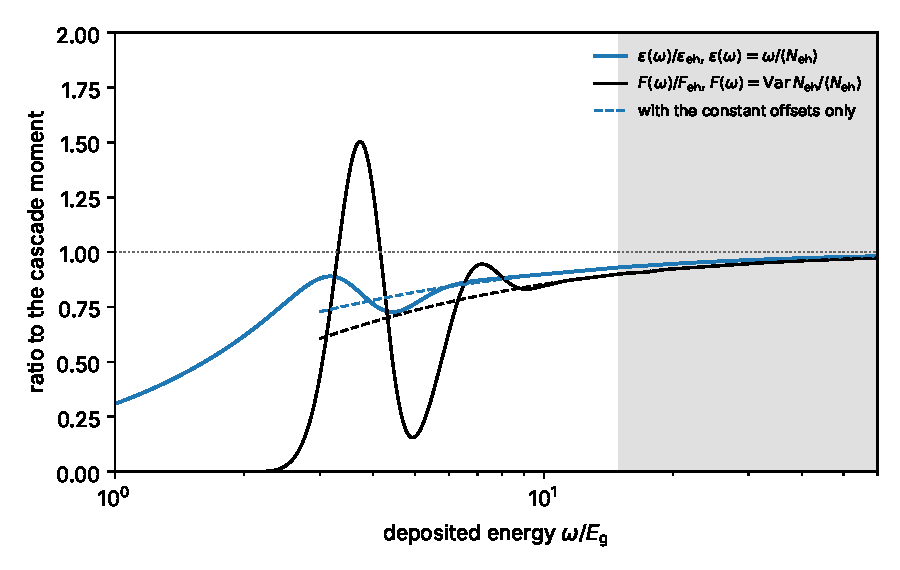
\includegraphics[width=\linewidth]{figures/ch18/limit18_2a.pdf}
\captionof{figure}{Pair energy (blue) and Fano factor (black) of a deposit $\omega$ in silicon, in units of their high-energy limits $\varepsilon_{\mathrm{eh}} = 3.232\,\Eg$ and $F_{\mathrm{eh}} = 0.114$, against $\omega/\Eg$. Energy-only random-$k$ cascade with $\Eg = \SI{1.160}{eV}$, $\omega_{\mathrm{AB}} = \SI{63}{meV}$, $A_{\mathrm{AB}} = \SI{5.703}{eV^3}$, $\theta_{\mathrm{ii}} = 1$, hole band width \SI{12}{eV}; seed electron with all of $\omega - \Eg$, hole at the band edge; moment recursions on a grid of step $\Eg/74$, the ratios taken on that grid. Dashed: the limits corrected by the constant terms only, $\varepsilon(\omega)/\varepsilon_{\mathrm{eh}} = (1 + b_N\varepsilon_{\mathrm{eh}}/\omega)^{-1}$ and $F(\omega)/F_{\mathrm{eh}} = (1 + c_N\varepsilon_{\mathrm{eh}}/F_{\mathrm{eh}}\omega)(1 + b_N\varepsilon_{\mathrm{eh}}/\omega)^{-1}$, with the constant terms of this seed fitted between 30 and $60\Eg$ ($b_N$ of \cref{sec:18.3-limits}, $c_N = -0.02$; the slopes are fitted between 20 and $40\Eg$). Gray: $\omega \ge 14.9\,\Eg = \SI{17.3}{eV}$, where both ratios lie within \SI{10}{\percent} of 1.}\label{fig:18-limit-moments}
\par}
\smallskip
Below about $15\Eg$ the yield rises in steps of one pair, and $F(\omega)$ swings between 0 and $1.5\,F_{\mathrm{eh}}$, so that a search at a few pairs needs the full distribution of the pair number (\cref{sec:18.3}) rather than two moments.
\end{limitbox}

At $\omega \le 2\Eg$ the seed electron cannot ionize and $F(\omega) = 0$: one pair, always. The first ionizations then make the variance rise and fall as each new pair becomes possible. Above $10\Eg$ the constant terms describe the approach to within \SI{1}{\percent}: at $\omega = 10\Eg$ the computed ratios differ from the dashed curves by \SI{0.07}{\percent} in $\varepsilon$ and \SI{0.9}{\percent} in $F$.

\subsection{The three variance terms in silicon}\label{sec:18.2-silicon}

In silicon the three terms of \cref{eq:18.2-decomp} are $\mathcal{V}_< = 0.092$, $\mathcal{V}_> = 0.290$ and $2\mathcal{V}_{<>} = -0.268$, and they add to $F_{\mathrm{eh}} = 0.114$. The largest term is not the residual energy below threshold but the phonon energy above it. The mean phonon energy emitted above threshold is \SI{0.92}{eV} per pair, about 15 phonons of \SI{63}{meV}. If those phonons were independent emissions, their number would be Poisson, $\operatorname{Var}E_> = \omega_{\mathrm{AB}}\langle E_>\rangle$, and $\mathcal{V}_> = w_{\mathrm{AB}}\langle E_>\rangle/(\Eg\bar n) = 0.043$. The computed term is 6.7 times larger. The reason is the steep energy dependence of \cref{eq:18.1-randomk}. Within a few phonon steps of threshold the probability that the next collision ionizes is below $10^{-4}$; it is 0.004 at \SI{2}{eV} and reaches a few percent only at 2.5 to \SI{3}{eV} (\cref{app:E.13}). As a result, a carrier in this range emits a run of phonons whose length has a long, nearly geometric tail. Two carriers that start at the same energy can end their runs many phonons apart.

Most of this variance is canceled by the covariance, which removes \SI{92}{\percent} of $\mathcal{V}_>$. Energy conservation along each carrier line ties the two heats together. A carrier that emits more phonons just above threshold either falls below threshold with a smaller residual, or ionizes later, at a lower energy, into smaller products. What a long run of phonons adds to $E_>$, it takes from $E_<$. The net Fano factor is therefore a small difference of two large terms, which has a practical consequence for any calculation: an error of \SI{1}{\percent} in $\mathcal{V}_>$ alone moves $F_{\mathrm{eh}}$ by \SI{2.5}{\percent}. The covariance is the correlation between the two kinds of heat along one line of descent, not between sibling carriers.

\Cref{fig:18-decomp} follows the three terms as phonon emission grows stronger, at the phonon step of silicon. Without phonons, $E_> = 0$ and $F_{\mathrm{eh}} = \mathcal{V}_<$ is pure partition noise: the scatter of the residual energies with which the carriers end, 0.081 for parabolic bands at $\theta_{\mathrm{ii}} = 1$. At $\lambda_{\mathrm{AB}} = 0.003$ the phonon term is still small, $\mathcal{V}_> = 0.009$, and the covariance is positive, $+0.010$. From $\lambda_{\mathrm{AB}} \approx 0.1$ on, both large terms grow, until at $\lambda_{\mathrm{AB}} = 30$ they reach $\mathcal{V}_> = 0.55$ and $2\mathcal{V}_{<>} = -0.61$. Across these four decades $F_{\mathrm{eh}}$ itself rises only from 0.085 to 0.132, and for $\lambda_{\mathrm{AB}}$ between 1 and 10 it stays between 0.105 and 0.122. In this model a Fano factor near 0.11 is generic for a semiconductor. A full-band cascade of silicon with no fitted constant gives the same 0.114 (\cref{sec:18.4-three}). The measured value tests the shape of the rate ratio within a few phonon energies of threshold, where the two large terms are made, more than it tests the constant $A_{\mathrm{AB}}$ (\cref{sec:18.4}).

\begin{figure}[tbp]
  \centering
  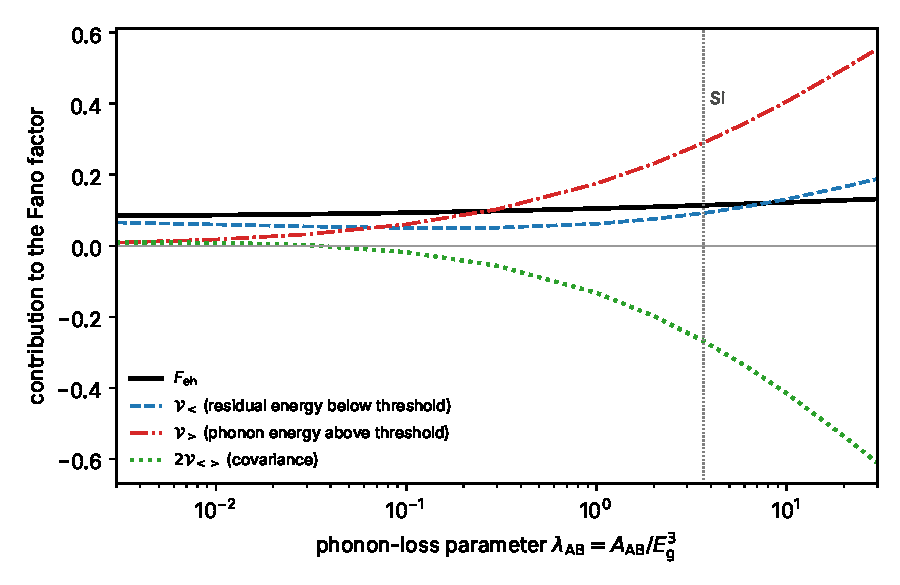
\includegraphics[width=0.85\linewidth]{figures/ch18/fig18_2.pdf}
  \caption{Fano factor $F_{\mathrm{eh}}$ (solid) and its three terms, \cref{eq:18.2-decomp}, against the phonon-loss parameter $\lambda_{\mathrm{AB}} = A_{\mathrm{AB}}/\Eg^3$ at the phonon step of silicon, $w_{\mathrm{AB}} = \omega_{\mathrm{AB}}/\Eg = 0.0543$. Dashed: $\mathcal{V}_<$, from the residual energies of the carriers when they fall below threshold; dash-dotted: $\mathcal{V}_>$, from the phonon energy emitted above threshold; dotted: $2\mathcal{V}_{<>}$, their covariance. Energy-only random-$k$ cascade with parabolic densities of states, $\theta_{\mathrm{ii}} = 1$, hole band width $12\,\mathrm{eV}/\Eg$; asymptotic slopes for seed energies between $X/2$ and $X$, $X = 40\Eg$ ($60\Eg$ for $\lambda_{\mathrm{AB}} > 5$); moment recursions on grids of step $\Eg/74$ and $\Eg/148$, extrapolated to zero step. The vertical line marks silicon, $\lambda_{\mathrm{AB}} = 3.654$, where the terms are $0.092 + 0.290 - 0.268 = 0.114$.}
  \label{fig:18-decomp}
\end{figure}

\subsection{The random-parking limit}\label{sec:18.2-parking}

One limit of the cascade has an exact solution. Take a constant electron density of states, a valence band so narrow that every hole is born at the band edge, $\theta_{\mathrm{ii}} = 1$, and no phonons. An electron of kinetic energy $x \ge \Eg$ then ionizes into a hole at rest and two electrons that share $x - \Eg$ with uniform probability, since the joint density of states of \cref{eq:18.1-phase} is flat on the line $x_1 + x_2 = x - \Eg$. In units of $\Eg$ this is the random parking problem of R\'enyi~\cite{subashiev2010correlation}. A car of unit length parks at a uniformly random place in a free gap of length $x$ and leaves two gaps, which are filled in the same way until every gap is shorter than a car. The jamming density $\rho_\infty$, the number of cars per unit length at the end, is the number of pairs per unit energy, so that $\varepsilon_{\mathrm{eh}} = \Eg/\rho_\infty$. Subashiev and Luryi proposed this limit as a test of Fano-factor models, since both moments are known exactly~\cite[Sect.~I]{subashiev2010correlation}. \Cref{we:18-parking} derives them from the recursions of \cref{sec:18.2-heat}.

\begin{workedexample}{The random-parking Fano factor}\label{we:18-parking}
Measure energies in units of $\Eg$. Let $M(x)$ be the mean number of new pairs made by an electron of kinetic energy $x$. The hole of each ionization is terminal with zero residual, and the two electrons share $x - 1$ uniformly, so \cref{eq:C.11-mean} with one pair per ionization reads $M(x) = 0$ for $x < 1$ and
\begin{equation*}
  M(x) = 1 + \frac{2}{x - 1}\int_0^{x - 1}M(y)\,\dd y , \qquad x \ge 1 .
\end{equation*}
Put $x = z + 1$ and multiply by $z$: $zM(z + 1) = z + 2\int_0^zM(y)\,\dd y$. Take the Laplace transform $m(s) = \int_0^\infty\ee^{-sx}M(x)\,\dd x$. Since $M$ vanishes below 1, the transform of $M(z + 1)$ is $\ee^sm(s)$, and multiplication by $z$ becomes $-\dd/\dd s$. With $\phi(s) = \ee^sm(s)$,
\begin{equation*}
  \phi'(s) + \frac{2\ee^{-s}}{s}\,\phi(s) = -\frac{1}{s^2} , \qquad
  \phi(s) = \int_s^\infty\frac{\dd t}{t^2}\,\exp\bigl[2E_1(s) - 2E_1(t)\bigr] ,
\end{equation*}
the solution that vanishes as $s \to \infty$, with $E_1(s) = \int_s^\infty\ee^{-u}u^{-1}\dd u$ the exponential integral. For every $s > 0$, exactly, $E_1(s) = -\gamma_{\mathrm{E}} - \ln s + \mathrm{Ein}(s)$, with Euler's constant $\gamma_{\mathrm{E}}$ and $\mathrm{Ein}(s) = \int_0^s(1 - \ee^{-u})u^{-1}\dd u \to 0$. Hence $\ee^{2E_1(s)} \to \ee^{-2\gamma_{\mathrm{E}}}/s^2$ as $s \to 0$, and inserting the same identity for $E_1(t)$ under the integral,
\begin{equation*}
  m(s) \to \frac{\rho_\infty}{s^2} , \qquad
  \rho_\infty = \int_0^\infty\exp\bigl[-2\,\mathrm{Ein}(t)\bigr]\,\dd t = 0.74759792 .
\end{equation*}
A double pole $\rho_\infty/s^2$ is the transform of $\rho_\infty x$, so $M(x) \to \rho_\infty x$: the pair energy is $\varepsilon_{\mathrm{eh}} = \Eg/\rho_\infty = 1.3376\,\Eg$. The second moment obeys \cref{eq:C.11-second} with the same kernel. Solved on grids of step 0.01 and 0.005 and extrapolated linearly in the step, it yields $F_{\mathrm{eh}} = 0.051040$ and $1/\varepsilon_{\mathrm{eh}} = 0.747599$, against the closed form $F_{\mathrm{park}} = 0.0510387$~\cite[Eq.~(44)]{subashiev2010correlation}.

The renewal estimate of \cref{sec:18.2-renewal} needs only the final state. At jamming, the number of gaps of size $g$ per unit length is~\cite[Eq.~(19)]{subashiev2010correlation}
\begin{equation*}
  G(g) = 2\int_0^\infty t\,\exp\bigl[-gt - 2\,\mathrm{Ein}(t)\bigr]\,\dd t , \qquad 0 \le g \le 1 .
\end{equation*}
Each gap is the residual energy of one terminal electron, and there is one per pair. Integrating, $\int G\,\dd g = \rho_\infty$ (one gap per car) and $\int(1 + g)G\,\dd g = 1$ (cars and gaps fill the line), both to 30 digits. Each pair costs $1 + g$, with $\langle g\rangle = 0.337617 = 1/\rho_\infty - 1$ and $\operatorname{Var}g = 0.079437$, so that \cref{eq:18.2-ren} gives
\begin{equation*}
  F_{\mathrm{ren}} = \frac{\operatorname{Var}g}{(1 + \langle g\rangle)^2} = 0.0443977 = 0.870\,F_{\mathrm{park}} .
\end{equation*}
The final-state statistics are exact here, and still the estimate misses \SI{13}{\percent} of the Fano factor. (The values printed in Ref.~\cite{subashiev2010correlation}, $\rho_\infty = 0.7475987$ and 0.0439766, carry misprints in the seventh and third digits.)
\end{workedexample}

Silicon is far from this limit in two ways. Its densities of states rise as $x^{1/2}$, and phonons compete with ionization. The density of states alone, at $\lambda_{\mathrm{AB}} \to 0$, raises $\varepsilon_{\mathrm{eh}}$ from $1.338\,\Eg$ to $1.585\,\Eg$ and $F_{\mathrm{eh}}$ from 0.051 to 0.081. \Cref{lim:18.2b} keeps the parking kernel and adds the phonons.

\begin{limitbox}[Random-parking limit][lim:18.2b]
For a constant electron density of states, holes born at the band edge, $\theta_{\mathrm{ii}} = 1$ and no phonons, the cascade is R\'enyi's random parking, with $\Eg/\varepsilon_{\mathrm{eh}} = \rho_\infty = \int_0^\infty\ee^{-2\,\mathrm{Ein}(t)}\dd t = 0.74759792$~\cite[Eq.~(23)]{subashiev2010correlation} and $F_{\mathrm{eh}} = F_{\mathrm{park}} = 0.0510387$~\cite[Eq.~(44)]{subashiev2010correlation}.
\par\smallskip
{\centering
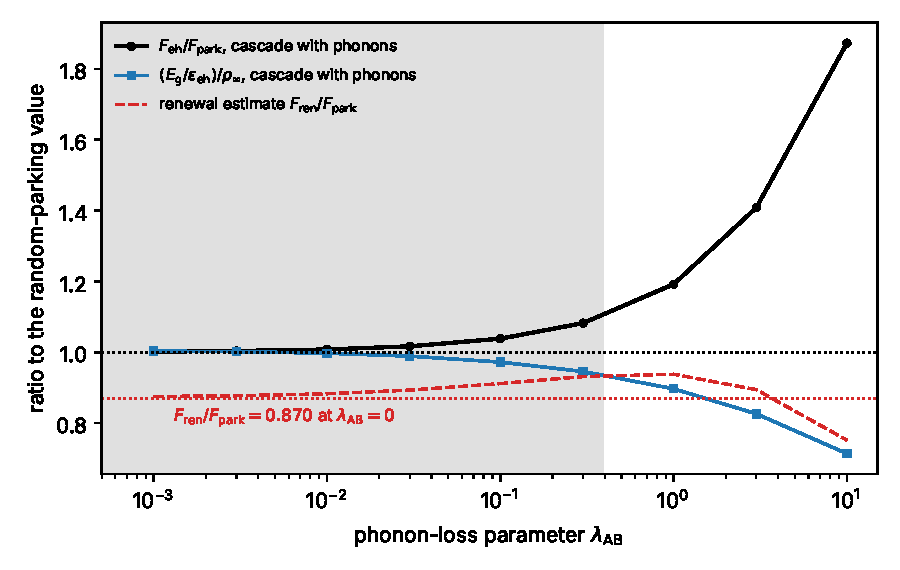
\includegraphics[width=\linewidth]{figures/ch18/limit18_2b.pdf}
\captionof{figure}{The parking kernel with phonons: $F_{\mathrm{eh}}/F_{\mathrm{park}}$ (black) and $(\Eg/\varepsilon_{\mathrm{eh}})/\rho_\infty$ (blue) against $\lambda_{\mathrm{AB}}$, with one phonon step $w_{\mathrm{AB}} = 0.0543$ (silicon) and the phonon-to-ionization ratio $\lambda_{\mathrm{AB}}/(x/\Eg - 1)$ of \cref{eq:18.1-randomk} for a constant density of states, where $\mathfrak{P}(y) = y$ and $A_{\mathrm{AB}}$ carries eV, so that here $\lambda_{\mathrm{AB}} = A_{\mathrm{AB}}/\Eg$. Dashed red: the renewal estimate $F_{\mathrm{ren}}$ of \cref{eq:18.2-rencasc}; dotted red: its parking value 0.870. Moment recursions on a grid of step $\Eg/74$, which places the values at $\lambda_{\mathrm{AB}} \to 0$ \SI{0.4}{\percent} ($\rho$) and \SI{0.1}{\percent} ($F$) above the exact ones. Gray: $\lambda_{\mathrm{AB}} < 0.40$, where both ratios are within \SI{10}{\percent} of 1 (bisection in $\ln\lambda_{\mathrm{AB}}$).}\label{fig:18-limit-park}
\par}
\smallskip
For $\lambda_{\mathrm{AB}} \gtrsim 0.4$ the carriers lose their last energy above threshold to phonons, which lowers the pair density and raises $F_{\mathrm{eh}}$, the trend that carries the parking values toward those of silicon.
\end{limitbox}

Relative to the parking values computed on the same grid, the phonons lower $\Eg/\varepsilon_{\mathrm{eh}}$ and raise $F_{\mathrm{eh}}$ by $0.8\,\lambda_{\mathrm{AB}}$ for $\lambda_{\mathrm{AB}} \le 0.003$, and by \SI{3.2}{\percent} and \SI{3.7}{\percent} at $\lambda_{\mathrm{AB}} = 0.1$. At $\lambda_{\mathrm{AB}} = 3$ the parking kernel leads to $F_{\mathrm{eh}} = 0.072$, 1.41 times $F_{\mathrm{park}}$; the rest of the way to the 0.114 of silicon is the shape of the densities of states.

\subsection{The renewal estimate}\label{sec:18.2-renewal}

A shortcut to $F_{\mathrm{eh}}$ uses only the statistics of the final state. Suppose that each pair costs the gap plus a heat $c_i$, that the costs are independent and identically distributed with mean $\varepsilon_{\mathrm{eh}} - \Eg$ and variance $\sigma_{\mathrm{pair}}^2$, and that pairs are made until $\omega$ is spent. This is the single renewal chain of \cref{app:C.11} with one loss per pair, and \cref{eq:C.11-fano} gives $\operatorname{Var}N_{\mathrm{eh}} \simeq \sigma_{\mathrm{pair}}^2\omega/\varepsilon_{\mathrm{eh}}^3$, that is,
\begin{equation}
  F_{\mathrm{ren}} = \frac{\sigma_{\mathrm{pair}}^2}{\varepsilon_{\mathrm{eh}}^2} ,
  \label{eq:18.2-ren}
\end{equation}
the uncorrelated final-state estimate of Subashiev and Luryi~\cite[Eq.~(7)]{subashiev2010correlation}. The denominator is $\varepsilon_{\mathrm{eh}}$, not $\Eg$. With $N_{\mathrm{eh}}$ held fixed, the heat would scatter by $\bar n\sigma_{\mathrm{pair}}^2$, and \cref{eq:18.2-moments} would give $\sigma_{\mathrm{pair}}^2/\Eg^2$. At fixed $\omega$, however, a pair that costs more heat leaves less energy for the pairs after it, and this constraint multiplies the variance by $(\Eg/\varepsilon_{\mathrm{eh}})^2$.

In a cascade the costs are built from computed statistics. Each pair ends with one terminal electron and one terminal hole, whose residual energies have the variances $\sigma_{\mathrm{e}}^2$ and $\sigma_{\mathrm{h}}^2$, and the phonon heat above threshold is taken as Poisson. Then
\begin{equation}
  F_{\mathrm{ren}} = \frac{\sigma_{\mathrm{e}}^2 + \sigma_{\mathrm{h}}^2 + \omega_{\mathrm{AB}}\langle E_>\rangle/\bar n}{\varepsilon_{\mathrm{eh}}^2} ,
  \label{eq:18.2-rencasc}
\end{equation}
which keeps the one-carrier statistics of the final state exactly and drops every correlation. In random parking it is the gap-law value 0.0443977 of \cref{we:18-parking}. \Cref{lim:18.2c} compares it with the full $F_{\mathrm{eh}}$.

\begin{limitbox}[Renewal estimate of the Fano factor][lim:18.2c]
For independent, identically distributed costs per pair with variance $\sigma_{\mathrm{pair}}^2$, the Fano factor is $F_{\mathrm{ren}} = \sigma_{\mathrm{pair}}^2/\varepsilon_{\mathrm{eh}}^2$~\cite[Eq.~(7)]{subashiev2010correlation}, built for the cascade as \cref{eq:18.2-rencasc}.
\par\smallskip
{\centering
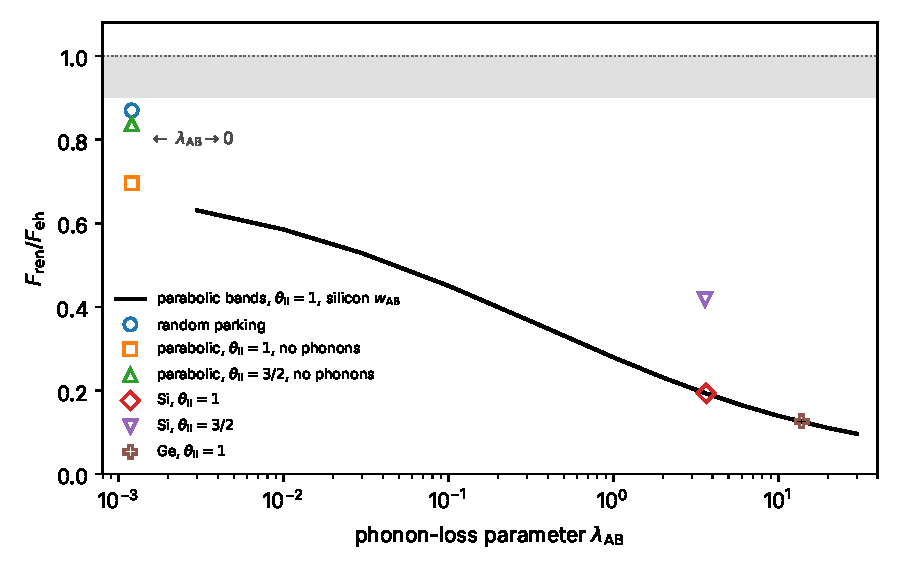
\includegraphics[width=\linewidth]{figures/ch18/limit18_2c.pdf}
\captionof{figure}{Ratio of the renewal estimate \cref{eq:18.2-rencasc} to the full Fano factor \cref{eq:18.2-decomp} against $\lambda_{\mathrm{AB}}$. Line: parabolic densities of states, $\theta_{\mathrm{ii}} = 1$, $w_{\mathrm{AB}} = 0.0543$, hole band width $12\,\mathrm{eV}/\Eg$ (the kernel of \cref{fig:18-decomp}). Markers at $\lambda_{\mathrm{AB}} \to 0$, extrapolated from grid steps 0.01 and $0.005\,\Eg$: random parking (0.870), parabolic bands without phonons at $\theta_{\mathrm{ii}} = 1$ (0.696) and $3/2$ (0.837). Further markers: silicon at $\theta_{\mathrm{ii}} = 1$ (0.193) and at $\theta_{\mathrm{ii}} = 3/2$ with $A_{\mathrm{AB}}$ recalibrated to the pair energy, \SI{5.629}{eV^3} (0.418); germanium with $\Eg = \SI{0.744}{eV}$, $\omega_{\mathrm{AB}} = \SI{37.6}{meV}$, the silicon $A_{\mathrm{AB}}$ and the hole density of states cut at the germanium valence-band width, \SI{12.6}{eV}~\cite[Table~II]{rideau2006strained} (0.126). Markers and line are continuum limits of the moment recursions. The gray band, within \SI{10}{\percent} of the full value, contains no computed case.}\label{fig:18-limit-renewal}
\par}
\smallskip
The estimate drops the correlations of the cascade, all of which raise the variance here: it lies below $F_{\mathrm{eh}}$ in every computed case, by \SI{13}{\percent} in random parking, by a factor 5 in silicon and by a factor 8 in germanium.
\end{limitbox}

The ratio falls from 0.70 to 0.10 as $\lambda_{\mathrm{AB}}$ grows, because the phonon heat above threshold is far from Poisson (\cref{sec:18.2-silicon}), while \cref{eq:18.2-rencasc} counts it as Poisson and has no covariance term at all. Without phonons the gap is smaller but still there: $F_{\mathrm{eh}} - F_{\mathrm{ren}} = 0.025$ at $\theta_{\mathrm{ii}} = 1$ and 0.013 at $\theta_{\mathrm{ii}} = 3/2$, with exact one-carrier statistics. This difference measures every departure from independent, identical costs together: correlations between the products of one ionization, between the electron and the hole of one pair, and between distant carriers, and the differences between the cost laws of different pairs. It does not isolate any one of them. In random parking Subashiev and Luryi find the correlation correction positive at intermediate filling and at jamming, and they note that correlations between the two halves of a split are not the only ones~\cite[Sect.~IV]{subashiev2010correlation}. A Fano factor fitted with a final-state model therefore needs a broader residual distribution, or a larger phonon variance, than the cascade actually has.

\subsection{The linear mean yield}\label{sec:18.2-linear}

The definitions \cref{eq:18.2-moments} assume that $\bar n$ grows in proportion to $\omega$. For a single chain of independent losses, \cref{app:C.11} proved this with the key renewal theorem, \cref{eq:C.11-linear}. The cascade is not a single chain, since an ionization splits the energy among three carriers, and no loss law is common to all its steps. The leading term still follows from renewal theory if we follow a unit of energy instead of a carrier. Give each ionization of a carrier at kinetic energy $x$ the weight 1, spread evenly over the $x$ units of energy that the carrier holds. The number of ionizations in a cascade started at kinetic energy $E$ is then the integral of the collected weights over all units. Taking the mean,
\begin{equation}
  \bar n_{\mathrm{sub}}(E) = E\,\Bigl\langle\sum_j\frac{1}{x_j}\Bigr\rangle_u ,
  \label{eq:18.2-tagged}
\end{equation}
where $u$ is a unit chosen uniformly in $[0, E]$, the sum runs over the ionizations along the chain of carriers that hold $u$, $x_j$ is the kinetic energy of the holder at the $j$-th of them, and $\langle\cdots\rangle_u$ is the mean over $u$ and over the cascade. A holder that emits phonons first ionizes below the energy at which it received the unit; $x_1 = E$ only if the first collision of the seed carrier is an ionization. The carriers that hold one unit form a chain. At an ionization the unit passes to one of the three products with probability equal to that product's share of the energy, or it leaves the chain into the gap of the new pair, with probability $\Eg/x$. At a phonon emission it leaves with probability $\omega_{\mathrm{AB}}/x$. \Cref{app:D.44} shows that \cref{eq:18.2-tagged} is exact for any branching law that conserves energy.

At high energy the shares no longer depend on $x$. In the random-$k$ model the products divide $x - \Eg$ in proportions whose law tends to a fixed law, and the probability of leaving into the gap falls as $\Eg/x$. The logarithm $\ln x_j$ thus performs a random walk with steps $\ln(x_{j+1}/x_j) \le 0$ whose law becomes independent of $x$. By the renewal theorem in the variable $\ln x$, the distribution with which the walk first arrives in the region within a few gaps of threshold converges as $E \to \infty$. The sum in \cref{eq:18.2-tagged} is dominated by that region, since the high-energy terms are small, $1/x_j$ each. Its mean converges. With the seed pair counted,
\begin{keyresult}[Linear mean yield]
\begin{equation}
  \bar n(\omega) = \frac{\omega}{\varepsilon_{\mathrm{eh}}} + o(\omega) , \qquad
  \frac{1}{\varepsilon_{\mathrm{eh}}} = \lim_{E\to\infty}\Bigl\langle\sum_j\frac{1}{x_j}\Bigr\rangle_u ,
  \label{eq:18.2-linear}
\end{equation}
for any energy-conserving cascade whose share law becomes independent of the energy at high energy, approaches that limit fast enough, is not concentrated on a lattice in $\ln x$, and is regular near threshold. \Cref{app:D.44} states the four conditions and gives the proof.
\end{keyresult}
\noindent The share law must be spread out in $\ln x$. A cascade that always splits in fixed proportions would make the walk lattice, and $\bar n/\omega$ would oscillate in $\ln\omega$ forever instead of converging.

Two statements that the definitions also use are not part of \cref{eq:18.2-linear}. The first is the constant term $b_N$, which depends on the seed (\cref{sec:18.3-limits}). In the one-phonon model every energy loss is a whole combination of $\Eg$ and $\omega_{\mathrm{AB}}$, and as for the deterministic chain of \cref{app:C.11} the constant then carries a periodic remainder that never dies out. We can therefore fit the slopes over a range of seed energies, $[X/2, X]$, which averages the remainder. The second is the linear growth of the variance, $\operatorname{Var}N_{\mathrm{eh}} = F_{\mathrm{eh}}\omega/\varepsilon_{\mathrm{eh}} + O(1)$, which the computed slopes obey but which needs the same second-order estimates as $b_N$.

\subsection{Constant term and the renewal bound}\label{sec:18.2-open}

The constant term and the variance of the yield at second order in renewal theory have not been derived for the branching cascade. The expansions $\bar n = \omega/\varepsilon_{\mathrm{eh}} + b_N + o(1)$ and $\operatorname{Var}N_{\mathrm{eh}} = F_{\mathrm{eh}}\omega/\varepsilon_{\mathrm{eh}} + O(1)$ need second-order estimates for the walk of \cref{eq:18.2-tagged} and the rate at which the cascade forgets its seed, and neither is in hand. The constant matters at a few pairs: at \SI{10}{eV} in silicon, $\omega/\varepsilon_{\mathrm{eh}} = 2.67$, and the constant term of the one-sided seed adds \SI{13}{\percent} to it. The second open question is whether the renewal estimate \cref{eq:18.2-rencasc} is a lower bound on $F_{\mathrm{eh}}$ for every cascade of this class. It is in every case computed here and in random parking, but there is no proof. A proof would make the final-state statistics a guaranteed floor for the Fano factor, and a counterexample would show which correlations can lower the variance.

\section{Seed distributions and the step model}\label{sec:18.3}

At $\omega = \SI{5}{eV}$ in silicon the step model of \cref{eq:1.5-step} puts every event in the two-pair bin. The cascade of \cref{sec:18.1}, with the constant calibrated in \cref{sec:18.4}, puts two pairs in \SI{17}{\percent} of the events started by a dark-matter kick at $q_0 = \alpha m_e$ and one pair in the rest. A search with a two-pair threshold therefore records about one in six of the \SI{5}{eV} events that the step model predicts. The cascade differs from the step model in two respects: how the \SI{3.84}{eV} above the gap is shared between the electron and the hole, and how often each carrier emits a phonon instead of ionizing at a few eV. The energy sharing and the phonon emission both enter through the hand-off \cref{eq:8.7-cond}. Once a final-state class has been turned into the energies of its two carriers, the generating function of \cref{sec:18.1} yields the whole pair-number distribution. The step model and a cascade seeded by a fixed split of the energy are limits of the pair-number distribution that replace the seed by a rule, and they fail in the few-pair bins, where the rule matters most.

\subsection{The seed distribution}\label{sec:18.3-seed}

A final-state class $\Lambda$ of the zero-phonon pair sector puts an electron at $E_{\mathrm{e}}(\Lambda)$ above the conduction minimum and a hole at $E_{\mathrm{h}}(\Lambda)$ below the valence maximum, with $E_{\mathrm{e}} + E_{\mathrm{h}} = \omega - \Eg$. In the energy-only reduction of \cref{sec:18.1-reductions} the cascade of the pair depends on these two energies; the crystal momenta $\vect{k} + \vect{q}$ and $\vect{k}$ matter only for the first collisions. Keeping the energies and dropping the momenta loses the first-generation memory that \cref{sec:18.1-reductions} locates. The input from the dark-matter interaction is then a distribution of carrier energies. The \emph{seed distribution} at momentum transfer $\vect{q}$, energy $\omega$ and velocity $\vect{v}$ is
\begin{equation}
  P_{\mathrm{seed}}(E_{\mathrm{e}},E_{\mathrm{h}}|\vect{q},\omega,\vect{v}) = \frac{\sum_\Lambda\sum_{a,b}\mathfrak{D}_{ab}(\vect{q},\vect{v})\,S_{ab}(\vect{q},\omega;\Lambda)\,\delta\bigl(E_{\mathrm{e}} - E_{\mathrm{e}}(\Lambda)\bigr)\,\delta\bigl(E_{\mathrm{h}} - E_{\mathrm{h}}(\Lambda)\bigr)}{\sum_{a,b}\mathfrak{D}_{ab}(\vect{q},\vect{v})\,S_{ab}(\vect{q},\omega)} ,
  \label{eq:18.3-seed}
\end{equation}
the probability density that the interaction leaves the electron at $E_{\mathrm{e}}$ and the hole at $E_{\mathrm{h}}$. The class-resolved responses add up to $S_{ab}(\vect{q},\omega)$ by \cref{eq:8.7-resolved}, so $P_{\mathrm{seed}}$ integrates to one when every class at $(\vect{q},\omega)$ is a pair, and to the pair share of the response otherwise; the other sectors seed their own cascades. A pair made together with a phonon of energy $\omega_{\vect{Q}}$ has $E_{\mathrm{e}} + E_{\mathrm{h}} = \omega - \omega_{\vect{Q}} - \Eg$, and the phonon energy goes to heat once (\cref{sec:8.7}). With one coupling row the seed distribution is independent of $\vect{v}$ and of the dark-matter model, as the class weights of \cref{sec:8.7-handoff} are; with several rows it depends on both. In the zero-phonon sector energy conservation leaves one variable, the electron's share $f_{\mathrm{e}} = E_{\mathrm{e}}/(\omega - \Eg)$ of the energy above the gap.

The generating function of \cref{eq:18.1-seed} turns the seed into a pair number. Keep only the pair-number variable, $s = \ee^{\lambda_N}$, and let $\mathfrak{G}_t(x;s)$ be the energy-only solution of \cref{eq:18.1-backward}: the generating function of the number of ionizations that a carrier of type $t$ at kinetic energy $x$ makes in its subtree. The seed pair is counted by the factor $s$, and the two subtrees are independent, so the cascade distribution of a class is the coefficient
\begin{equation}
  P_{\mathrm{casc}}(N_{\mathrm{eh}}|\Lambda) = [s^{N_{\mathrm{eh}}}]\;s\,\mathfrak{G}_{\mathrm{e}}\bigl(E_{\mathrm{e}}(\Lambda);s\bigr)\,\mathfrak{G}_{\mathrm{h}}\bigl(E_{\mathrm{h}}(\Lambda);s\bigr) ,
  \label{eq:18.3-pcasc}
\end{equation}
where $[s^n]$ takes the coefficient of $s^n$. The cascade distribution depends on $\Lambda$ only through the two carrier energies. Write $P_{\mathrm{casc}}(N_{\mathrm{eh}}|\Lambda)$ as $\int\dd E_{\mathrm{e}}\,\dd E_{\mathrm{h}}\,\delta(E_{\mathrm{e}} - E_{\mathrm{e}}(\Lambda))\,\delta(E_{\mathrm{h}} - E_{\mathrm{h}}(\Lambda))\,P_{\mathrm{casc}}(N_{\mathrm{eh}}|E_{\mathrm{e}},E_{\mathrm{h}})$ inside the class sum of \cref{eq:8.7-cond}, and exchange the sum with the integral. The class sum then becomes the numerator of \cref{eq:18.3-seed}:
\begin{equation}
  P(N_{\mathrm{eh}}|\vect{q},\omega,\vect{v}) = \int\dd E_{\mathrm{e}}\,\dd E_{\mathrm{h}}\;P_{\mathrm{seed}}(E_{\mathrm{e}},E_{\mathrm{h}}|\vect{q},\omega,\vect{v})\;P_{\mathrm{casc}}(N_{\mathrm{eh}}|E_{\mathrm{e}},E_{\mathrm{h}}) .
  \label{eq:18.3-pq}
\end{equation}
The generating function of \cref{eq:18.3-pq} is $s\int P_{\mathrm{seed}}\,\mathfrak{G}_{\mathrm{e}}\mathfrak{G}_{\mathrm{h}}$, a power series with nonnegative coefficients that converges on $|s| \le 1$. The discrete Fourier sum \cref{eq:E.24-dft} of this generating function at $N_z$ roots of unity returns $\sum_jP(N_{\mathrm{eh}} + jN_z)$, the exact probability once $N_z$ exceeds every pair number with appreciable weight.

The backward recursion alone guarantees three things: the pair-number distribution is normalized, it is exactly one pair below $(1 + \theta_{\mathrm{ii}})\Eg$, and its variance splits into a cascade part and a seed part. First, each $\mathfrak{G}_t$ is a probability generating function, because the recursion of \cref{eq:18.1-backward} maps products and mixtures of generating functions to generating functions; \cref{eq:18.3-pq} is then normalized and nonnegative. Second, below $\theta_{\mathrm{ii}}\Eg$ no carrier ionizes, $\mathfrak{G}_t = 1$, and $P_{\mathrm{casc}} = \delta_{N_{\mathrm{eh}}1}$ exactly. The first ionization becomes possible at $\omega = (1 + \theta_{\mathrm{ii}})\Eg$, which is \SI{2.32}{eV} in silicon with $\theta_{\mathrm{ii}} = 1$, for a seed that gives all the energy to one carrier. Third, the moments separate the cascade from the seed. Let $m_t(x)$ and $v_t(x)$ be the mean and variance of the number of ionizations in one subtree, and let $\langle\cdot\rangle_{\mathrm{seed}}$ average over $P_{\mathrm{seed}}$. The law of total variance gives
\begin{equation}
  \langle N_{\mathrm{eh}}\rangle = 1 + \bigl\langle m_{\mathrm{e}}(E_{\mathrm{e}}) + m_{\mathrm{h}}(E_{\mathrm{h}})\bigr\rangle_{\mathrm{seed}} , \qquad
  \operatorname{Var}N_{\mathrm{eh}} = \bigl\langle v_{\mathrm{e}} + v_{\mathrm{h}}\bigr\rangle_{\mathrm{seed}} + \operatorname{Var}_{\mathrm{seed}}\bigl(m_{\mathrm{e}} + m_{\mathrm{h}}\bigr) .
  \label{eq:18.3-moments}
\end{equation}
The second term of the variance is the spread of the subtree means over the seed. It vanishes when $m_{\mathrm{e}} + m_{\mathrm{h}}$ takes one value on the whole support of the seed, for a single split and in the forced region $\omega < (1 + \theta_{\mathrm{ii}})\Eg$, where both means are zero.

$P_{\mathrm{seed}}$ is the per-pair weight of \cref{eq:8.7-IP} or of the screened form \cref{eq:8.7-screened}, binned in the two carrier energies; a library of computed responses stores $P_{\mathrm{seed}}$ in this binned form. With the functions $\mathfrak{G}_t$ tabulated on an energy grid, the seeded distribution costs one integral per momentum transfer, energy and pair of coupling rows.

\subsection{Pair-number distributions in silicon}\label{sec:18.3-silicon}

\Cref{fig:18-pn10} shows \cref{eq:18.3-pq} at $\omega = \SI{10}{eV}$ for six seeds run through one cascade. The cascade is the random-$k$ model of \cref{sec:18.1-reductions} with the silicon parameters of \cref{sec:18.2-heat}. The dark-matter seed comes from the empirical-pseudopotential bands of \cref{we:8-pairs}: the pair weights of the density at $\vect{q}_0 = \alpha m_e\hat{\vect{x}}$, without screening. The photon seed is the optical limit of the same bands. The model bands have a gap of \SI{0.82}{eV}, so each band seed is taken at the same excess energy $\omega - \Eg$ as the cascade uses. To compare two pair-number distributions we use the total-variation distance $d_{\mathrm{TV}}(P,Q) = \tfrac12\sum_N|P(N) - Q(N)|$, which is the largest difference between the probabilities that the two distributions assign to any set of pair numbers, for instance to the events above a search threshold. Screening hardly moves the energy shares: at \SI{10}{eV} the screened out-state seed of \cref{we:8-pairs} and its unscreened counterpart give distributions with $d_{\mathrm{TV}} = 0.010$.

\begin{figure}[tbp]
  \centering
  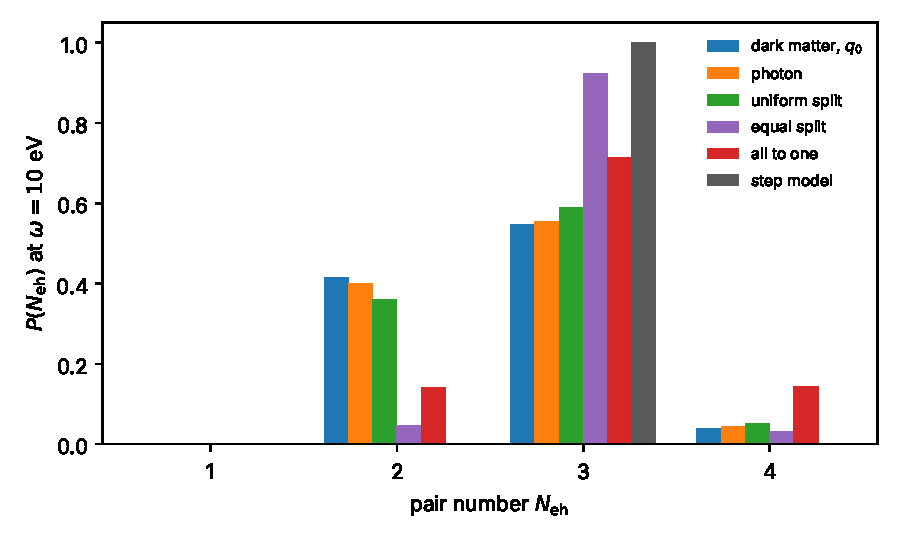
\includegraphics[width=0.85\linewidth]{figures/ch18/fig18_3.pdf}
  \caption{Pair-number distribution $P(N_{\mathrm{eh}})$ at $\omega = \SI{10}{eV}$ in silicon, \cref{eq:18.3-pq}, for six seeds in one cascade: the energy-only random-$k$ model of \cref{sec:18.1-reductions} with $\Eg = \SI{1.160}{eV}$, $\omega_{\mathrm{AB}} = \SI{63}{meV}$, $\theta_{\mathrm{ii}} = 1$, holes below \SI{12}{eV} and $A_{\mathrm{AB}} = \SI{5.703}{eV^3}$, calibrated to $\varepsilon_{\mathrm{eh}} = \SI{3.749}{eV}$. The band seeds are a dark-matter kick at $q_0 = \alpha m_e$ along [100] (independent-particle pair weights of the density, empirical-pseudopotential bands of \cref{we:8-pairs}) and an absorbed photon (optical limit of the same bands). The other four seeds are the fixed splits of \cref{sec:18.3-limits} (uniform, equal, and all the energy to one carrier) and the step model \cref{eq:1.5-step} with $\varepsilon_{\mathrm{eh}} = \SI{3.749}{eV}$. Band seeds are used at the excess energy $\omega - \Eg$ of the model bands, whose gap is \SI{0.82}{eV}. Means: 2.626 (dark matter), 2.645 (photon), 2.691, 2.985 and 3.003 (the three splits), 3 (step model). $P(1)$ and $P(5)$ are below 0.002 for every seed. Probabilities from the generating function at $N_z = 32$ roots of unity; no distribution in this section has a mean above six.}
  \label{fig:18-pn10}
\end{figure}

The dark-matter seed yields two pairs with probability 0.414, three with 0.547 and four with 0.039. The mean, 2.626 pairs, corresponds to \SI{3.81}{eV} per pair, \SI{1.6}{\percent} above the high-energy pair energy. The photon seed yields 0.400, 0.555 and 0.045, and its mean is 2.645. The step model puts every event in the three-pair bin; it overstates the mean by \SI{14}{\percent} and misses the two-pair bin entirely. Of the three splits of \cref{sec:18.1-seed}, the equal split puts three pairs in \SI{92}{\percent} of events, the uniform split behaves like the band seeds, and giving everything to one carrier fills the four-pair bin with probability 0.143.

The variance shows where the seed enters. For the dark-matter seed \cref{eq:18.3-moments} splits $\operatorname{Var}N_{\mathrm{eh}} = 0.314$ into 0.283 from the subtrees and 0.031 from the spread of the seed. The equal split has no seed term, and its variance is 0.079, a quarter of the band-seed value. The subtree mean is far from linear in the share: at $f_{\mathrm{e}} = \tfrac14$, \SI{2.21}{eV} on one carrier and \SI{6.63}{eV} on the other, the two carriers make 2.436 pairs, against 2.985 at the equal split and 3.003 with all \SI{8.84}{eV} on one carrier. A carrier at \SI{2.21}{eV} almost never ionizes, while one at \SI{4.42}{eV} usually does once, so the count depends on how many carriers end up a little above \SI{4}{eV}.

\begin{workedexample}{The step model against the cascade at 5 eV}\label{we:18-step5}
Take $\omega = \SI{5}{eV}$ in silicon with the constants of \cref{fig:18-pn10}. The step model puts $N_{\mathrm{eh}} = 1 + \lfloor(5 - 1.160)/3.749\rfloor = 1 + \lfloor1.024\rfloor = 2$ pairs for every event; the literature values $\Eg = \SI{1.11}{eV}$ and $\varepsilon_{\mathrm{eh}} = \SI{3.6}{eV}$ of \cref{sec:1.5} give 2 as well.

In the cascade, the pair shares $\omega - \Eg = \SI{3.84}{eV}$. Consider first a seed that gives all of it to one carrier. Below $\Eg$ the carrier cannot ionize; above, the probability that its next collision is an ionization is $p_{\mathrm{ii}}(E) = [1 + \varGamma_{\mathrm{ph}}/\varGamma_{\mathrm{ii}}]^{-1}$ from \cref{eq:18.1-randomk}. The ionization probability is 0.0041 at \SI{2}{eV}, 0.0184 at \SI{2.5}{eV}, 0.049 at \SI{3}{eV}, 0.100 at \SI{3.5}{eV} and 0.145 at \SI{3.84}{eV}. As long as the carrier does not ionize, it walks down in steps of $\omega_{\mathrm{AB}}$: from \SI{3.84}{eV} it makes 43 collisions above $\Eg$. The probability that none of them is an ionization is
\begin{equation*}
  P_{\mathrm{no}} = \prod_{k=0}^{42}\bigl[1 - p_{\mathrm{ii}}(3.84\,\mathrm{eV} - k\,\omega_{\mathrm{AB}})\bigr] = 0.176 .
\end{equation*}
Replacing the sum of $-\ln(1 - p_{\mathrm{ii}}) \approx p_{\mathrm{ii}}/(1 - p_{\mathrm{ii}})$ over steps by an integral over energy, $\ln P_{\mathrm{no}} \approx -\omega_{\mathrm{AB}}^{-1}\int_{\Eg}^{3.84\,\mathrm{eV}}\dd E\;\varGamma_{\mathrm{ii}}/\varGamma_{\mathrm{ph}} = -1.735$, which leads to the same 0.176. If the carrier does ionize, the three products share at most $3.84 - 1.16 = \SI{2.68}{eV}$, and a second ionization follows with probability 0.002. This seed therefore leaves one pair with probability 0.176 and two with 0.822. A seed that splits the energy equally leaves two carriers at \SI{1.92}{eV}, each of which escapes ionization with probability 0.990, so that \SI{98}{\percent} of events end with one pair.

The dark-matter seed at $q_0$ lies between the one-sided seed and the equal split. At this energy the electron takes \SI{2.08}{eV} of the \SI{3.84}{eV} on average, and \SI{26}{\percent} of the weight has one carrier with more than three quarters of the energy. Averaging $P_{\mathrm{no}}(E_{\mathrm{e}})P_{\mathrm{no}}(E_{\mathrm{h}})$ over the seed in \cref{eq:18.3-pq} yields
\begin{equation*}
  P(1) = 0.831 , \qquad P(2) = 0.169 , \qquad P(3) = 6\times10^{-5} ,
\end{equation*}
a mean of 1.169 pairs and \SI{4.28}{eV} per pair. Above a two-pair threshold the step model therefore counts 5.9 times as many \SI{5}{eV} events as this cascade does; the full-band cascade of \cref{sec:18.3-fullband} raises the factor to about ten. The photon seed has $P(2) = 0.190$, \SI{12}{\percent} more than the dark-matter seed.
\end{workedexample}

\subsection{The full-band cascade as reference}\label{sec:18.3-fullband}

Every distribution so far comes from the energy-only cascade with its one constant fitted to the measured pair energy. A cascade with no fitted constant replaces the random-$k$ kernels by the kernels of \cref{sec:18.1} on full bands, in the standard full-band Monte Carlo form~\cite{fischetti1988monte}. In the calculation we use as reference, the bands are the empirical pseudopotential bands of Cohen and Bergstresser~\cite{cohen1966band}, with the form factors refit to measured transition energies; impact ionization is the golden rule with the diagonal, statically screened Coulomb kernel~\cite{cappellini1993model}, its direct and exchange terms combined as in Kane's form quoted by Kotani and van Schilfgaarde~\cite[Eq.~(5)]{kotani2010impact}; and phonon emission uses the deformation potentials and phonon energies of Refs.~\cite{lundstrom2000fundamentals,jacoboni1983monte}, \cite[Table~III]{li2021deformation}; the gap is $\Eg = \SI{1.160}{eV}$. The seeds are the pairs a dark-matter particle with a heavy mediator leaves in the same bands, with their crystal momenta. The calculation is varied jointly over the screening (static and dynamic), the phonon couplings (these values against first-principles ones, which weigh electron losses by 0.52 and hole losses by 3.0) and the exchange factor near threshold (0.5 to 1.0), and the ranges below are the envelope of these variants, for pair probabilities with the error of the $\vect{k}$ grid added.

At \SI{5}{eV} the full-band cascade puts two or more pairs in a fraction $0.097$ of the dark-matter events, with the envelope $[0.030, 0.173]$, against the 0.169 of the energy-only cascade in \cref{we:18-step5}. The step model, which puts every event in the two-pair bin, then overcounts that bin about tenfold, and at least sixfold anywhere in the envelope; the thirtyfold end of the envelope comes from one extreme corner alone, static screening of the weaker kind with tripled hole couplings and the lowest exchange factor. The energy-only cascade remains the working model of this chapter, because it is calibrated and fast. Recalibrated to the pair energy of each full-band variant, so that only the shape of the kernels differs, the energy-only cascade lies 0.12 to 0.20 in $d_{\mathrm{TV}}$ from the full-band distribution between 6 and \SI{8}{eV}. The soft onset of impact ionization near threshold matters most in this range, and the distance grows with the pair energy of the variant. On the same footing the uniform split lies 0.11 to 0.12 away, the equal split 0.45 to 0.50 and the step model 0.79 to 0.83.

\subsection{Fixed splits and the step limit}\label{sec:18.3-limits}

A fixed split replaces the seed distribution of \cref{eq:18.3-pq} by a distribution of the electron's share $f_{\mathrm{e}}$ that is the same for every process at a given $\omega$ and symmetric under the exchange of electron and hole. Three fixed splits bracket the range: all the energy on one carrier, a uniform share, and the equal split. The constant term $b_N$ of the mean (\cref{sec:18.2-heat}) depends on the seed. In the cascade of \cref{fig:18-pn10}, with $\omega/\varepsilon_{\mathrm{eh}}$ subtracted at the pair energy of the same calculation, it is 0.008 for the uniform split and 0.35 for a seed that gives all the energy to one carrier.

The step model is the limit in which every pair has a fixed cost. Let the first pair cost $\Eg$ and every further one exactly $\varepsilon_{\mathrm{eh}}$. The energy $\omega - \Eg$ left after the first pair is then spent by a renewal chain with the deterministic loss $\varepsilon_{\mathrm{eh}}$, which fits $\lfloor(\omega - \Eg)/\varepsilon_{\mathrm{eh}}\rfloor$ losses (\cref{app:C.11}). The pair number is
\begin{equation}
  N_{\mathrm{eh}}^{\mathrm{step}}(\omega) = 1 + \left\lfloor\frac{\omega - \Eg}{\varepsilon_{\mathrm{eh}}}\right\rfloor , \qquad P_{\mathrm{casc}}(N_{\mathrm{eh}}|\Lambda) = \delta_{N_{\mathrm{eh}},N_{\mathrm{eh}}^{\mathrm{step}}(\omega)} ,
  \label{eq:18.3-step}
\end{equation}
which is \cref{eq:1.5-step}, with a Fano factor of zero. Both the seed and the competition with phonons have been replaced by one cost per pair. In the forced region, $\omega < (1 + \theta_{\mathrm{ii}})\Eg$, the step model is exact. Above the forced region, even the mean is wrong. Over one period of $\omega$ the floor function loses $\tfrac12$ on average (\cref{app:C.11}), so the step model has the mean $(\omega - \Eg)/\varepsilon_{\mathrm{eh}} + \tfrac12 = \omega/\varepsilon_{\mathrm{eh}} + 0.19$ in silicon, against $\omega/\varepsilon_{\mathrm{eh}} + b_N$ in the cascade, with $b_N$ between 0.008 and 0.35 depending on the seed. This error in the mean falls as $1/\langle N_{\mathrm{eh}}\rangle$. The step-model distribution itself never approaches the cascade distribution. For a single bin $n$ the distance $d_{\mathrm{TV}}$ is $1 - P(n)$. The cascade distribution spreads over a width $\sigma_N = (F_{\mathrm{eh}}\omega/\varepsilon_{\mathrm{eh}})^{1/2}$ that grows with $\omega$: at \SI{20.2}{eV} the computed distribution of the dark-matter seed has $\sigma_N = 0.79$ and its largest bin holds 0.45, so the step model misplaces more than half of the events there, and the misplaced fraction grows with the width.

\Cref{lim:18.3a} compares each phenomenological seed with the dark-matter seed from the gap to \SI{21}{eV}, the range of the few-pair bins in silicon.

\begin{limitbox}[Step model and fixed splits][lim:18.3a]
The step model is \cref{eq:18.3-step}~\cite[Eq.~(5.1)]{essig2016direct}; the three fixed splits above are each run through the cascade by \cref{eq:18.3-pcasc}.
\par\smallskip
{\centering
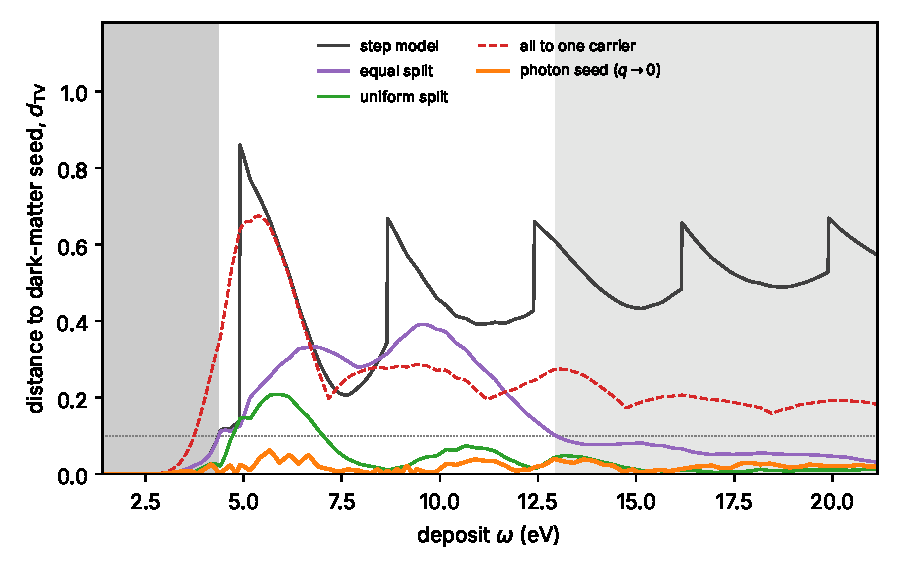
\includegraphics[width=\linewidth]{figures/ch18/limit18_3a.pdf}
\captionof{figure}{Distance $d_{\mathrm{TV}}$ between the pair-number distribution of each phenomenological seed and the distribution of the dark-matter seed at $q_0 = \alpha m_e$ along [100], against the deposit $\omega$ in silicon. All seeds run through one cascade, the energy-only random-$k$ model of \cref{sec:18.1-reductions} with $\Eg = \SI{1.160}{eV}$, $\omega_{\mathrm{AB}} = \SI{63}{meV}$, $\theta_{\mathrm{ii}} = 1$, holes below \SI{12}{eV} and $A_{\mathrm{AB}} = \SI{5.703}{eV^3}$. Black: step model, $\varepsilon_{\mathrm{eh}} = \SI{3.749}{eV}$. Purple, green and red dashed: the equal split, the uniform split and all the energy to one carrier, with the seeds that put a hole above \SI{12}{eV} removed. Orange: the photon ($q \to 0$) seed of the same empirical-pseudopotential bands as the dark-matter seed. Band seeds are computed every \SI{0.25}{eV} of the excess energy $\omega - \Eg$ (model gap \SI{0.82}{eV}) and interpolated linearly; the curves use a \SI{0.02}{eV} grid. Dark gray: $\omega < \SI{4.37}{eV}$, where the step model and the uniform and equal splits are within 0.1 of the dark-matter seed. Light gray: $\omega > \SI{12.95}{eV}$, where the uniform and equal splits are again within 0.1 of the dark-matter seed. Dotted: $d_{\mathrm{TV}} = 0.1$.}\label{fig:18-limit-seed}
\par}
\smallskip
Between \SI{4.4}{eV} and \SI{13}{eV} the split of the energy decides the count, so the split must come from the bands and the operator that made the pair. There the uniform and equal splits reach distances of 0.21 and 0.39, the one-sided split 0.67, and the step model is off by up to 0.86 at its first step, $\omega = \Eg + \varepsilon_{\mathrm{eh}} = \SI{4.91}{eV}$.
\end{limitbox}

Below \SI{4.37}{eV} the step model and the fixed splits hold because few carriers ionize: the dark-matter seed leaves one pair with probability above 0.9, and so does any split that avoids putting the whole energy on one carrier. The distance of the step model exceeds 0.1 from \SI{4.37}{eV} on: at its first step the step model moves every event into the two-pair bin while the cascade puts 0.14 there, and its distance stays above 0.2 up to \SI{21}{eV}, above 0.39 beyond \SI{9}{eV}. The uniform and equal splits come within 0.04 of the dark-matter seed at \SI{21}{eV}. The one-sided split stays 0.18 away even there. At \SI{21}{eV} the valence band no longer holds the whole energy, so this split can put the energy only on the electron, and its mean lies 0.36 pairs above the mean of the dark-matter seed. A shift of the mean by a fixed amount gives a distance that decreases only as $\sigma_N^{-1} \propto \omega^{-1/2}$.

The photon seed is the case that matters in practice, because a photon calibration measures it, and the difference between the photon seed and the dark-matter seed is the error that \cref{sec:8.7-handoff} left open. In the energy-only cascade, with both seeds from the same band calculation on one $\vect{k}$ grid, the photon seed stays within 0.062 of the dark-matter seed everywhere, with the largest distance at \SI{5.67}{eV}, where the means differ by \SI{4.6}{\percent}. At \SI{10}{eV} the distance is 0.014, and above \SI{15}{eV} it is at most 0.03. These distances are internal to the energy-only model. They measure only the difference of the energy shares and carry the error of the photon seed's $\vect{k}$ grid: in the full-band calculation of \cref{sec:18.3-fullband} the photon seed moves by 0.11 to 0.14 between grids, as much as its distance from the dark-matter seed, so the full-band value of this distance is unresolved. The energy-only reduction drops the valleys and crystal momenta of the first generation, which the dark matter populates differently from a photon; a calculation that keeps the valleys and crystal momenta would add their share of the error. Absorption of a dark photon has no error from substituting the photon seed, because the absorbed dark photon leaves the same seed as a photon (\cref{sec:8.7-handoff}).

\subsection{Pair number at the readout}\label{sec:18.3-observable}

Every distribution so far is the distribution of the pair number at the end of the prompt cascade, about a picosecond after the deposit, when every carrier has reached its band edge. A detector reads the event microseconds to seconds later, and what it reads depends on more than the pair number. The induced charge depends on where the pairs are and how far each carrier drifts. Capture costs one gap per captured electron, and excitons change the measured Fano factor (\cref{sec:18.5}). A phonon readout records the heat with its spectrum. The cascade therefore records, besides $N_{\mathrm{eh}}$, further quantities $\mathfrak{m}$: the positions of the carriers at the end of the prompt cascade, the electron and hole counts separately, the spectrum of the emitted phonons and the energy stored in defects. Let $P_{\mathrm{det}}(\mathsf{R}|N_{\mathrm{eh}},\mathfrak{m})$ be the probability that the readout records $\mathsf{R}$, a charge, a phonon energy or both, at the time it reads. The distribution of the recorded quantity for an event of class $\Lambda$ is
\begin{equation}
  P_{\mathrm{obs}}(\mathsf{R}|\Lambda) = \sum_{N_{\mathrm{eh}}}\int\dd\mathfrak{m}\;P_{\mathrm{casc}}(N_{\mathrm{eh}},\mathfrak{m}|\Lambda)\;P_{\mathrm{det}}(\mathsf{R}|N_{\mathrm{eh}},\mathfrak{m}) ,
  \label{eq:18.3-obs}
\end{equation}
and it replaces $P_{\mathrm{casc}}$ in \cref{eq:8.7-handoff} when the rate is written for the recorded quantity. The quantities $\mathfrak{m}$ are read off the same cascade sample as the pair number, so the generating function of \cref{eq:18.1-backward} carries them as further components of the deposit.

The step model and \cref{eq:18.3-pq} are statements about one marginal of \cref{eq:18.3-obs}: the pair number at the end of the prompt cascade, with $P_{\mathrm{det}} = \delta_{\mathsf{R}N_{\mathrm{eh}}}$. Every later process acts on that marginal and on $\mathfrak{m}$ together. If each pair is collected independently with probability $f_{\mathrm{det}}$, the recorded number is thinned binomially, its Fano factor is $f_{\mathrm{det}}F_{\mathrm{eh}} + 1 - f_{\mathrm{det}}$ by \cref{eq:C.11-thinfano}, and $\mathfrak{m}$ drops out. If collection depends on position or on the carrier type, $\mathfrak{m}$ does not drop out, and the rate needs the joint law. \Cref{sec:18.5} treats the second factor of \cref{eq:18.3-obs} up to the end of the cascade; the readout itself is the subject of \cref{chap:20}.

\section{Calibrated pair energies}\label{sec:18.4}

Back at keV deposits, where two moments describe the pair number, a charge-resolving silicon sensor at \SI{123}{K} measures $\varepsilon_{\mathrm{eh}} = \SI{3.749 \pm 0.001}{eV}$ and $F_{\mathrm{eh}} = 0.119 \pm 0.002$ for \SI{5.9}{keV} X-rays~\cite{rodrigues2021absolute}. The cascade of \cref{sec:18.1,sec:18.2}, reduced to energy alone and given free-particle kernels, has one constant that a measurement must fix. Once the measured $\varepsilon_{\mathrm{eh}}$ fixes the constant, the cascade predicts $F_{\mathrm{eh}}$. It predicts both numbers for every other crystal as well, including the crystals ranked in \cref{chap:17}, for most of which neither number has been measured. A guide to new targets needs a pair energy for each crystal, and it needs to know which of these pair energies rest on comparison with data. With its one constant fixed in silicon, the cascade comes within 5 to \SI{6}{\percent} of the measured pair energies of germanium and GaAs, and its pair energies reduce to the line $\varepsilon_{\mathrm{eh}} \approx 1.61\Eg + k_2$.

\subsection{The calibrated cascade}\label{sec:18.4-model}

The model is the random-$k$ cascade of \cref{sec:18.1-reductions} with free-particle densities of states, threshold ratio $\theta_{\mathrm{ii}} = 1$, one optical phonon of energy $\omega_{\mathrm{AB}}$ and, in silicon, a hole band cut at $B_{\mathrm{h}} = \SI{12}{eV}$, solved by the moment recursions of \cref{sec:18.2-heat}. In units of the gap the model depends on a crystal through the two numbers defined in \cref{sec:18.2-heat}, the phonon strength $\lambda_{\mathrm{AB}} = A_{\mathrm{AB}}/\Eg^3$ and the phonon step $w_{\mathrm{AB}} = \omega_{\mathrm{AB}}/\Eg$. A cascade with large $\lambda_{\mathrm{AB}}$ loses most of its energy to phonons on the way down and settles more slowly: germanium, with $\lambda_{\mathrm{AB}} > 5$, needs slopes fitted for seed energies between 30 and $60\Eg$, against 20 to $40\Eg$ for silicon. All values are the continuum limit of the recursions.

The constant is fixed in silicon. With $\Eg = \SI{1.160}{eV}$ at \SI{123}{K}~\cite[Eq.~(11)]{ramanathan2020ionization} and $\omega_{\mathrm{AB}} = \SI{63}{meV}$, the measured pair energy requires
\begin{equation}
  A_{\mathrm{AB}} = \SI{5.703}{eV^3} ,
  \label{eq:18.4-AAB}
\end{equation}
so that $\lambda_{\mathrm{AB}} = 3.65$ and $w_{\mathrm{AB}} = 0.0543$ for silicon. The same constant leads to $F_{\mathrm{eh}} = 0.114$ (\cref{sec:18.2-silicon}). This value of $A_{\mathrm{AB}}$ lies \SI{10}{\percent} above the 5.2 that Alig and coworkers fitted to the pair energy of silicon~\cite[Sect.~II]{nielsen2026first}. With 5.2 and the room-temperature gap of \SI{1.12}{eV}, the same cascade gives \SI{3.64}{eV}, inside the range of 3.62 to \SI{3.66}{eV} measured at \SI{300}{K}~\cite[Table~I]{ramanathan2020ionization}. Everything else in this section uses \cref{eq:18.4-AAB} unchanged: one constant for all crystals. The universality of the constant is an assumption, and the comparison with other crystals tests it.

Two cascade calculations with no constant left to fit exist for silicon. Nielsen and Fischetti use density-functional bands and phonons, a loss-function kernel without exchange and a plasmon channel, and find $\varepsilon_{\mathrm{eh}} = \SI{3.10}{eV}$ with a time-dependent density-functional loss function and \SI{3.50}{eV} with a $GW$/Bethe--Salpeter one~\cite[Sect.~III]{nielsen2026first}; they apply the same method to six of the crystals below (the last column of \cref{tab:18-valid}). The full-band cascade of \cref{sec:18.3-fullband} uses empirical pseudopotential bands and deformation-potential phonons and gives $\varepsilon_{\mathrm{eh}} = \SI{4.15}{eV}$, with the envelope $[3.95, 4.73]$~eV of its variants. The class of model adds a systematic of at least $\pm\SI{0.4}{eV}$, taken from the shift between the two loss functions of Nielsen and Fischetti. Without a fitted constant, Nielsen and Fischetti lie below the measured \SI{3.749}{eV} and the full-band cascade above it. The two calculations do not meet even with matched ingredients: with first-principles phonon couplings for both carriers and without exchange, as Nielsen and Fischetti have them, the full-band cascade still gives \SI{4.11}{eV}, and the remaining difference of \SI{0.6}{eV} from their \SI{3.50}{eV} is unexplained. The unexplained difference lies where the pair energy is decided, in the rate of impact ionization between threshold and about \SI{4.5}{eV} (\cref{sec:18.1-reductions}). At \SI{100}{eV} the full-band cascade turns \SI{71.6}{\percent} of the deposit into heat, with the envelope $[70.2, 75.0]$~\si{\percent}.

\subsection{Silicon, germanium and GaAs}\label{sec:18.4-three}

\Cref{tab:18-pairs} sets the model against the measurements. Each crystal is computed twice: at the gap of the measurement temperature, for the comparison, and at its low-temperature gap of \cref{tab:3-materials}, for a detector at millikelvin. Temperature enters the model only through $\Eg(T)$. Leaving out phonon absorption costs little: the occupation of the \SI{37.6}{meV} germanium phonon is 0.0035 at \SI{77}{K}. The phonon energy $\omega_{\mathrm{AB}}$ is the measured zone-center optical energy, \SI{37.6}{meV} for germanium (\cref{tab:5-phonons}) and the longitudinal \SI{36.35}{meV} for GaAs (\cref{sec:5.5}); neither crystal has a hole cutoff.

\begin{table}[tbp]
\caption{Mean energy per pair and Fano factor of the energy-only random-$k$ cascade with the single constant \cref{eq:18.4-AAB}, against measurements. Germanium gap at \SI{77}{K} from the fit of Wei, Wang and Mei~\cite[Eq.~(7)]{wei2016average}; other gaps from \cref{tab:3-materials} and \cref{app:E.13}. Measurements: silicon~\cite{rodrigues2021absolute}; germanium, the pair energy and the range of five Fano-factor experiments quoted by Mei and coworkers~\cite[Sect.~4.3]{mei2020impact}; GaAs, the room-temperature value of Bertuccio and Maiocchi as quoted by Nielsen and Fischetti~\cite[Fig.~1]{nielsen2026first}. Residual: model over measured, minus one.}
\label{tab:18-pairs}
\centering\small\setlength{\tabcolsep}{4pt}
\begin{tabular}{llccccc>{\raggedright\arraybackslash}p{0.2\linewidth}}
\toprule
 & $T$ & $\Eg$ (eV) & \multicolumn{2}{c}{$\varepsilon_{\mathrm{eh}}$ (eV)} & \multicolumn{2}{c}{$F_{\mathrm{eh}}$} & Status \\
 & & & model & measured & model & measured & \\
\midrule
Si & \SI{123}{K} & 1.160 & 3.749 & $3.749 \pm 0.001$ & 0.114 & $0.119 \pm 0.002$ & $\varepsilon$ fitted; $F$ predicted, $2.4\sigma$ low \\
 & low & 1.17 & 3.766 & -- & 0.114 & -- & model \\
Ge & \SI{77}{K} & 0.735 & 2.815 & 2.96 & 0.125 & 0.06--0.13 & $\varepsilon$ residual $-\SI{4.9}{\percent}$; $F$ inside the spread \\
 & low & 0.744 & 2.831 & -- & 0.124 & -- & model \\
GaAs & \SI{300}{K} & 1.42 & 3.964 & $\approx 4.2$ & 0.104 & -- & $\varepsilon$ residual $-\SI{5.6}{\percent}$ \\
 & low & 1.52 & 4.132 & -- & 0.102 & -- & model \\
\bottomrule
\end{tabular}
\end{table}

In silicon the pair energy is fitted, and the Fano factor is the test. The model yields $F_{\mathrm{eh}} = 0.114$, $2.4\sigma$ below $0.119 \pm 0.002$, with no uncertainty assigned to the model; the temperature dependence measured by Lowe and Sareen implies $0.118 \pm 0.004$ at \SI{123}{K}, as quoted in the same work~\cite{rodrigues2021absolute}, about $1\sigma$ above the model. The test is stronger than it looks, because $F_{\mathrm{eh}}$ hardly depends on the fitted constant. Raising $A_{\mathrm{AB}}$ by \SI{10}{\percent} raises $\varepsilon_{\mathrm{eh}}$ by \SI{1.2}{\percent} and $F_{\mathrm{eh}}$ by \SI{0.65}{\percent}; the secant slopes at the silicon gap are $\partial\varepsilon_{\mathrm{eh}}/\partial A_{\mathrm{AB}} = \SI{0.076}{eV^{-2}}$ and $\partial F_{\mathrm{eh}}/\partial A_{\mathrm{AB}} = \SI{0.0013}{eV^{-3}}$. At fixed constant the slope in the gap is $\partial\varepsilon_{\mathrm{eh}}/\partial\Eg = 1.70$. The calibration leaves $F_{\mathrm{eh}}$ where the structure of the model puts it, and the structural choices move it more than the constant does. Recalibrated with the impact-ionization threshold at $\frac32\Eg$ instead of $\Eg$, the model gives 0.113; with a density of states rising as $x$ instead of $x^{1/2}$, 0.102. Neither choice reaches 0.119. Nor does the full-band cascade of \cref{sec:18.3-fullband}, which has no fitted constant: it gives $F_{\mathrm{eh}} = 0.114$, with the envelope $[0.101, 0.115]$ of its variants, and no variation within its class moves $F_{\mathrm{eh}}$ toward the measurement. The energy-only model and the full-band cascade both leave out the plasmon channel, excitonic final states and momentum-dependent phonon couplings, so their agreement does not show that the difference between 0.114 and the measured 0.119 is structural. $F_{\mathrm{eh}}$ is set within a few phonon energies of threshold (\cref{sec:18.2-silicon}), where the free-particle form of \cref{eq:18.1-randomk} is least reliable.

Germanium tests the pair energy. With the constant fixed in silicon, the model yields \SI{2.81}{eV} at \SI{77}{K}, a residual of $-\SI{4.9}{\percent}$ against the measured \SI{2.96}{eV}~\cite[Sect.~4.3]{mei2020impact}. The larger phonon strength of germanium, $\lambda_{\mathrm{AB}} = 14.4$ against 3.65 for silicon, puts $\varepsilon_{\mathrm{eh}}$ at $3.83\Eg$, against $3.23\Eg$ in silicon. The measured Fano factors of germanium scatter from 0.06 to 0.13~\cite[Sect.~4.3]{mei2020impact}, a spread wider than the model's own sensitivity, so the model value 0.125 is consistent with the data but not tested by them. No germanium pair energy has been measured at millikelvin; the value that a bolometric detector uses rests on extrapolation from \SI{77}{K}~\cite{wei2016average}, and the model's \SI{2.83}{eV} at the low-temperature gap is itself an extrapolation.

GaAs is the polar contrast. Its pair energy has been measured at room temperature, about \SI{4.2}{eV} by Bertuccio and Maiocchi as quoted by Nielsen and Fischetti~\cite[Fig.~1]{nielsen2026first}, against the model's \SI{3.96}{eV}, a residual of $-\SI{5.6}{\percent}$. With $\lambda_{\mathrm{AB}} = 1.99$ and $w_{\mathrm{AB}} = 0.026$, GaAs loses less energy to phonons than silicon, and $\varepsilon_{\mathrm{eh}} = 2.79\Eg$. The optical phonons of GaAs couple to the carriers through the long-range Fr\"ohlich field, which the constant matrix element of \cref{eq:18.1-randomk} does not distinguish from the short-range deformation-potential coupling of silicon. The strongly unequal electron and hole masses of GaAs and its $\mathrm{\Gamma}$, $\mathrm{L}$ and $\mathrm{X}$ conduction valleys make a single parabolic random-$k$ kernel especially crude. No Fano factor of GaAs has been measured. The residuals of germanium and GaAs are both negative: with the silicon constant, the model puts too little heat into each pair in these two crystals.

\subsection{The linear law of the pair energy}\label{sec:18.4-linear}

In the reduced cascade every pair ends with exactly one terminal electron and one terminal hole: the seed's hole starts at the band edge, and each ionization adds one pair and one carrier of each kind. Let $\bar E_{\mathrm{res}}$ be the mean residual energy per terminal carrier and $r_K$ the mean number of phonons of energy $\omega_K = \omega_{\mathrm{AB}}$ emitted above threshold per pair. The residual heat $E_<$ and the phonon heat $E_>$ of \cref{sec:18.2-heat} then have means $2\bar E_{\mathrm{res}}\bar n$ and $r_K\omega_K\bar n$, and dividing the energy identity $\omega = N_{\mathrm{eh}}\Eg + E_< + E_>$ by $\bar n$ at large $\omega$ gives
\begin{equation}
  \varepsilon_{\mathrm{eh}} = \Eg + 2\bar E_{\mathrm{res}} + r_K\omega_K .
  \label{eq:18.4-shockley}
\end{equation}
This is Shockley's energy balance, with his threshold energy replaced by the gap in the pair term~\cite[Eq.~(1)]{nielsen2026first}. In silicon the computed terms are $1.160 + 1.666 + \SI{0.923}{eV} = \SI{3.749}{eV}$: the residual energy per carrier is $\bar E_{\mathrm{res}} = 0.718\Eg$, and each pair carries 14.6 phonons emitted above threshold. Without phonons, $\lambda_{\mathrm{AB}} \to 0$, the cascade yields $\varepsilon_{\mathrm{eh}} = 1.585\Eg$ with $\bar E_{\mathrm{res}} = 0.293\Eg$: each ionization splits the available energy three ways in proportion to the joint density of states, and the products that land below threshold land mostly near the band edge, as in random parking (\cref{sec:18.2-parking}). A carrier that emits phonons near threshold reaches its last ionization with less energy to spare and more often stalls just above threshold, so $\bar E_{\mathrm{res}}$ grows with $\lambda_{\mathrm{AB}}$.

Measured pair energies are fitted by straight lines in the gap, $\varepsilon_{\mathrm{eh}} = k_1\Eg + k_2$~\cite[Sect.~I]{nielsen2026first}. The most recent fit, dominated by wide-gap crystals, is $1.54\Eg + \SI{1.89}{eV}$~\cite[Sect.~II]{nielsen2026first}. The cascade explains why a straight line fits and why its constant term differs from crystal to crystal. Over the fit region $0.003 \le \lambda_{\mathrm{AB}} \le 100$, $0.01 \le w_{\mathrm{AB}} \le 0.1$, which contains 13 of the 24 crystals of \cref{chap:17}, sixty solutions of the cascade are reproduced by
\begin{equation}
  \frac{\varepsilon_{\mathrm{eh}}}{\Eg} = 1.612 + 2.329\,\bigl(\lambda_{\mathrm{AB}}\,w_{\mathrm{AB}}^{0.9637}\bigr)^{0.2403} ,
  \label{eq:18.4-fit}
\end{equation}
to \SI{0.61}{\percent} at most and \SI{0.21}{\percent} on average (\cref{fig:18-limit-c}). \Cref{eq:18.4-fit} is an observed fit of the model, not a derivation; its exponents carry no meaning beyond the fit region. Inserting $\lambda_{\mathrm{AB}} = A_{\mathrm{AB}}/\Eg^3$ turns it into a nearly linear law in the gap, because the power of $\Eg$ in the second term, $1 - (3 + 0.9637)\times0.2403 = 0.048$, is almost zero:
\begin{equation}
  \varepsilon_{\mathrm{eh}} \approx 1.61\,\Eg + k_2 , \qquad
  k_2 = 2.329\,\bigl(A_{\mathrm{AB}}\,\omega_{\mathrm{AB}}^{0.9637}\bigr)^{0.2403}\,\Eg^{0.048} ,
  \label{eq:18.4-linear}
\end{equation}
energies in eV and $A_{\mathrm{AB}}$ in eV$^3$. The slope is the phonon-free part of the pair energy at the random-$k$ threshold, 1.61 against the exact 1.585 above; the constant $k_2$ is the phonon loss. Since $A_{\mathrm{AB}}$ is the same for all crystals, $k_2$ depends on the phonon energy, as $\omega_{\mathrm{AB}}^{0.23}$, and only weakly on the gap. For silicon it is \SI{1.88}{eV}. Over the 24 crystals of \cref{chap:17} it spans 1.21 to \SI{2.53}{eV}, and 1.51 to \SI{2.53}{eV} for those inside the fit region: soft lattices, with small $\omega_{\mathrm{AB}}$, lose less to phonons, and stiff ones more.

\begin{limitbox}[Linear law of the pair energy][lim:18.4c]
The observed linear law of the cascade, \cref{eq:18.4-linear}, $\varepsilon_{\mathrm{eh}} \approx 1.61\Eg + k_2$ with $k_2 = 1.2$ to \SI{2.5}{eV}, agrees in form with the empirical fit $\varepsilon_{\mathrm{eh}} = 1.54\Eg + \SI{1.89}{eV}$~\cite[Sect.~II]{nielsen2026first}.
\par\smallskip
{\centering
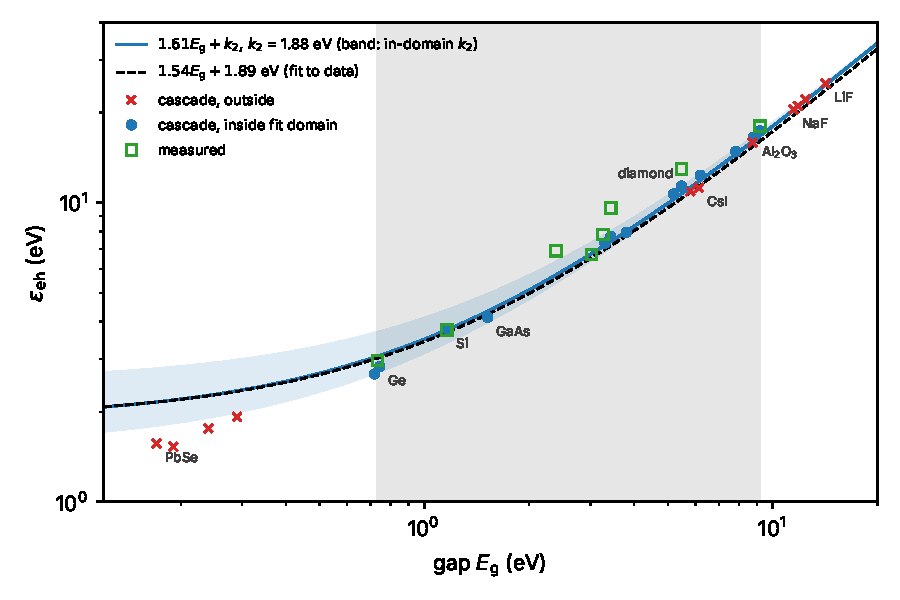
\includegraphics[width=\linewidth]{figures/ch18/limit18_4c.pdf}
\captionof{figure}{Pair energy against the gap. Solid line: \cref{eq:18.4-linear} with the silicon value $k_2 = \SI{1.88}{eV}$; band: $k_2$ over the crystals inside the fit region, 1.51 to \SI{2.53}{eV}. Dashed: the empirical line. Circles: the cascade with the constant \cref{eq:18.4-AAB} for the 24 crystals of Griffin and coworkers~\cite[Table~I]{griffin2020multichannel} (gap and highest optical phonon energy; silicon, germanium and GaAs at their low-temperature gaps of \cref{tab:3-materials}); filled inside the fit region $0.003 \le \lambda_{\mathrm{AB}} \le 100$, $0.01 \le w_{\mathrm{AB}} \le 0.1$ of \cref{eq:18.4-fit}, crosses outside it. Squares: measured pair energies of \cref{tab:18-valid} and silicon. Gray: the gaps of the measured crystals, 0.73 to \SI{9.2}{eV}. Slopes fitted for seed energies of 12.5 to $25\Eg$ (30 to $60\Eg$ for $\lambda_{\mathrm{AB}} > 5$), a window that changes the silicon value by less than \SI{0.03}{\percent} against the 20 to $40\Eg$ of \cref{tab:18-pairs}.}\label{fig:18-limit-c}
\par}
\smallskip
Outside the fit region, the law with each crystal's own $k_2$ still follows the cascade to \SI{1.4}{\percent} for these 24 crystals, but there it extrapolates the model beyond any comparison with data: the lead salts and InSb have $\lambda_{\mathrm{AB}} > 200$, and the halides and fluorides a phonon step below $0.006\Eg$.
\end{limitbox}

The linear law of the cascade and the empirical line have the same form for different reasons. The empirical constant 1.89 lies inside the range of $k_2$ and close to the value for silicon. The empirical slope 1.54 is below the model's 1.61, pulled down by diamond and the nitrides, for which the model with the silicon constant gives too little (\cref{sec:18.4-range}). Nielsen and Fischetti note that the measured $\varepsilon_{\mathrm{eh}}(\Eg)$ is not linear~\cite[Sect.~II]{nielsen2026first}; in the model, the nonlinearity comes from $k_2$, which changes from crystal to crystal with the phonon energy.

\begin{workedexample}{Pair energy of GaAs from the linear law}\label{we:18-gaas}
A GaAs detector at millikelvin has $\Eg = \SI{1.52}{eV}$ (\cref{tab:3-materials}) and a longitudinal optical phonon at $\omega_{\mathrm{AB}} = \SI{36.35}{meV}$ (\cref{sec:5.5}). With \cref{eq:18.4-AAB},
\begin{equation*}
  \lambda_{\mathrm{AB}} = \frac{5.703}{1.52^3} = 1.624, \qquad w_{\mathrm{AB}} = \frac{0.03635}{1.52} = 0.02391 .
\end{equation*}
The combination in \cref{eq:18.4-fit} is $\lambda_{\mathrm{AB}}w_{\mathrm{AB}}^{0.9637} = 0.04448$, and its power $0.2403$ is 0.4733. Then
\begin{equation*}
  \frac{\varepsilon_{\mathrm{eh}}}{\Eg} = 1.612 + 2.329\times0.4733 = 2.714, \qquad
  \varepsilon_{\mathrm{eh}} = 2.714\times\SI{1.52}{eV} = \SI{4.125}{eV} .
\end{equation*}
In the form \cref{eq:18.4-linear}, $1.61\Eg = \SI{2.45}{eV}$ and $k_2 = \SI{1.68}{eV}$, smaller than silicon's \SI{1.88}{eV} because the GaAs phonon carries 0.58 of the silicon phonon energy. The cascade itself yields \SI{4.132}{eV} (\cref{tab:18-pairs}), so the fit costs \SI{0.2}{\percent}. The empirical line gives \SI{4.23}{eV}. At the room-temperature gap of \SI{1.42}{eV} the linear law gives \SI{3.96}{eV}, against the measured value of about \SI{4.2}{eV}~\cite[Fig.~1]{nielsen2026first}; the difference is the residual of the model in \cref{tab:18-pairs}, carried through the fit. For a GaAs detector the defensible pair energy is therefore $\approx\SI{4.1}{eV}$ with an uncertainty set by the model's residuals, not by the fit.
\end{workedexample}

\subsection{The validated range}\label{sec:18.4-range}

\Cref{tab:18-valid} compares the cascade with the measured pair energies of seven crystals besides silicon, which fixes the constant. The inputs are the gap and the highest optical phonon energy of each crystal, longitudinal for the SiC polytypes.

\begin{table}[tbp]
\caption{Pair energies of the cascade with the silicon constant \cref{eq:18.4-AAB} against measurements. Inputs: germanium as in \cref{tab:18-pairs} (\SI{77}{K}); diamond, GaN and $\alpha$-quartz, gap and highest optical phonon energy of Griffin and coworkers~\cite[Table~I]{griffin2020multichannel}; the SiC polytypes, gap and longitudinal optical energy of Griffin and coworkers~\cite[Table~I]{griffin2021sic}. Measurements: germanium~\cite[Sect.~4.3]{mei2020impact}; diamond, the inverse-variance mean of four measurements (13.1, 13.25, 13.05 and \SI{12.82}{eV}) compiled by Nielsen and Fischetti~\cite[Sect.~III]{nielsen2023thermalization}; 4H-SiC~\cite{gsponer2023measurement}; 6H-SiC as quoted by Griffin and coworkers~\cite[Table~I]{griffin2021sic}; 3C-SiC and SiO$_2$ as quoted by Nielsen and Fischetti~\cite[Table~II]{nielsen2026first}; GaN, electron-beam induced current, as quoted by Nielsen and coworkers~\cite[Sect.~IV]{nielsen2023first}. Residual: model over measured, minus one. Last column: the density-functional full-band Monte Carlo of Nielsen and coworkers~\cite[Table~II]{nielsen2026first}, \cite[Sect.~III]{nielsen2023thermalization}, \cite[Sect.~IV]{nielsen2023first}.}
\label{tab:18-valid}
\centering\footnotesize\setlength{\tabcolsep}{3pt}
\begin{tabular}{lcccccccc}
\toprule
 & $\Eg$ (eV) & $\omega_{\mathrm{AB}}$ (meV) & $\lambda_{\mathrm{AB}}$ & $w_{\mathrm{AB}}$ & model (eV) & measured (eV) & residual & full band (eV) \\
\midrule
Ge & 0.735 & 37.6 & 14.4 & 0.051 & 2.815 & 2.96 & $-\SI{4.9}{\percent}$ & -- \\
3C-SiC & 2.39 & 120.5 & 0.42 & 0.050 & 6.121 & 6.90 & $-\SI{11.3}{\percent}$ & 6.6 \\
6H-SiC & 3.02 & 120.0 & 0.21 & 0.040 & 7.167 & 6.7 & $+\SI{7.0}{\percent}$ & -- \\
4H-SiC & 3.26 & 120.0 & 0.16 & 0.037 & 7.565 & $7.83 \pm 0.02$ & $-\SI{3.4}{\percent}$ & 7.3 \\
GaN & 3.43 & 88.9 & 0.14 & 0.026 & 7.694 & 9.59 & $-\SI{19.8}{\percent}$ & 8.9 \\
diamond & 5.47 & 161 & 0.035 & 0.029 & 11.357 & 12.95 & $-\SI{12.3}{\percent}$ & 12.87 \\
SiO$_2$ & 9.2 & 149 & 0.0073 & 0.016 & 17.373 & 18.0 & $-\SI{3.5}{\percent}$ & 16.7 \\
\bottomrule
\end{tabular}
\end{table}

Over the seven crystals the residuals run from $-\SI{19.8}{\percent}$ to $+\SI{7.0}{\percent}$, with a mean of $-\SI{6.9}{\percent}$ and a root mean square of \SI{10.5}{\percent}. The model is good to \SI{7}{\percent} for germanium, 4H- and 6H-SiC and quartz, and it falls short by 11 to \SI{20}{\percent} for 3C-SiC, diamond and GaN. Six of the seven residuals are negative, as are the residuals of germanium and GaAs in \cref{tab:18-pairs}: with the silicon constant the model tends to give too little heat per pair. The likeliest cause of the negative residuals is the universal constant, since the light-atom and polar lattices that the model misses most have phonon couplings unlike the couplings of silicon, but the comparison does not prove that the constant is the cause. The density-functional full-band Monte Carlo does better for diamond, 3C-SiC and GaN and worse for 4H-SiC and quartz, and it has no fitted constant. Its \SI{3.1}{eV} for silicon (\cref{sec:18.4-model}), \SI{17}{\percent} below the \SI{3.749}{eV} at \SI{123}{K}, shows that it is not yet a calibration-free substitute either.

The Fano factor is barely tested beyond silicon. The germanium measurements span a factor two, and the only wide-gap values, both for 4H-SiC, disagree with each other: $F_{\mathrm{eh}} = 0.1$ from a linewidth and an upper limit of 0.04 from another, as compiled by Gsponer and coworkers~\cite[Table~2]{gsponer2023measurement}. The model gives 0.093 for 4H-SiC. If the upper limit holds, the model fails for 4H-SiC, since 0.04 lies below every Fano factor the cascade produces in this section; a linewidth limit, however, rests on subtracting the noise from the measured width~\cite[Eq.~(3)]{gsponer2023measurement}, and an overestimated noise drives the limit down. Which of the two 4H-SiC values applies cannot be decided from the published data.

These comparisons define the \emph{validated range} of the cascade model: the region of phonon strength and phonon step spanned by the crystals with a measured pair energy, $0.007 \le \lambda_{\mathrm{AB}} \le 14.4$ and $0.016 \le w_{\mathrm{AB}} \le 0.054$, gaps from 0.73 to \SI{9.2}{eV}. Inside the validated range a model pair energy carries the spread of the residuals, $-20$ to $+\SI{7}{\percent}$, with the lower part more likely for light-atom and polar crystals. Of the crystals ranked in \cref{chap:17}, silicon, germanium, GaAs, diamond, quartz, CaWO$_4$, AlN, GaN and ZnO lie inside the range (\cref{fig:18-limit-c}). Sapphire and MgO lie just outside, with phonon steps of 0.012 and 0.011, and GaSb at its edge, with $\lambda_{\mathrm{AB}} = 15.3$.

Three groups lie well outside the validated range. The alkali halides and the fluorides, NaI, CsI, NaCl, LiF, NaF, CaF$_2$ and MgF$_2$, have phonon steps of 0.0016 to 0.006 of the gap. A carrier near threshold then emits hundreds of phonons before it ionizes, and no measured crystal samples a regime with so many phonons per ionization. The halides and fluorides have narrow anion valence bands, which confine the holes far more than in any validated crystal and which the model treats without a cutoff. They also bind excitons by an eV or more. A carrier between $\Eg - E_x^b$ and the impact-ionization threshold can create a bound pair directly; the cascade of \cref{sec:18.1} has no channel for this direct exciton creation, and whether a bound exciton counts as a pair depends on the readout (\cref{sec:18.5}). The lead salts and InSb have gaps below \SI{0.3}{eV} and $\lambda_{\mathrm{AB}}$ from 230 to 1160: their cascades are dominated by phonons, and at gaps this small, two processes absent from the model, Auger recombination and scattering by free carriers, can compete with impact ionization. For the crystals of these three groups the model pair energies in \cref{fig:18-limit-c} are estimates without a measured anchor, for example \SI{25.0}{eV} for LiF, \SI{20.5}{eV} for NaF, \SI{11.2}{eV} for CsI and \SI{1.56}{eV} for PbSe. Any guide to new targets must mark these pair energies as estimates. Neither the pair energy nor the Fano factor of sapphire, CaWO$_4$, LiF or NaF has been measured.

\section{Capture and excitons}\label{sec:18.5}

A carrier in silicon whose kinetic energy has fallen below the impact-ionization threshold $\theta_{\mathrm{ii}}\Eg$ (\cref{sec:18.1}) can no longer add a pair. It reaches the band edge by emitting phonons within about a picosecond, and from then on the number of pairs $N_{\mathrm{eh}}$ whose mean and variance \cref{sec:18.2} computes is fixed. A detector at \SI{50}{mK} reads the event microseconds to seconds later. In that interval an electron can be captured by an ionized donor, or an electron and a hole can bind into an exciton. The exciton can bind to a neutral impurity, and the pair can recombine, giving its energy to the lattice or to a photon that leaves the crystal. Each of these processes changes what a charge or a heat readout records, and none of their rates has been measured at millikelvin temperatures in silicon or germanium. Without the rates one can still derive how each process changes the energy balance and the pair number.

\subsection{End-of-cascade capture}\label{sec:18.5-capture}

At the end of the cascade every carrier sits at a band edge, and the deposit is shared by the energy balance \cref{eq:18.1-energy}: $\Eg$ for each pair and the heat $E_{\mathrm{heat}}$ for the phonons emitted on the way down. This holds for an electron recoil, with no energy stored in defects and no photon leaving the crystal. Once carriers can be captured, not all of the energy outside the pairs is heat, and we name it separately,
\begin{equation}
  E_{\mathrm{np}} \equiv \omega - N_{\mathrm{eh}}\Eg ,
  \label{eq:18.5-Enp}
\end{equation}
the energy not held by pairs, equal to $E_{\mathrm{heat}}$ as long as nothing is captured. At fixed $\omega$ the pair number and $E_{\mathrm{np}}$ fluctuate together, $\operatorname{Var}N_{\mathrm{eh}} = \operatorname{Var}E_{\mathrm{np}}/\Eg^2$. From here on $N_{\mathrm{eh}}$ counts the electrons in the conduction band, free or bound to a hole in an exciton. An electron captured on an impurity level no longer counts.

Let an electron be captured on a level $E_j$ below the conduction-band edge $E_c$. The energy of a charge in the crystal is fixed relative to the Fermi level $\mu_F$ of the electrodes, since that is the energy the carrier gives up when it reaches one. A free electron holds $E_c - \mu_F$, a free hole $\mu_F - E_v$, with $E_v$ the valence-band edge, and a pair the sum, $\Eg$. After the capture the electron holds $E_j - \mu_F$, the phonons emitted at capture carry $E_c - E_j$, and the hole, now without a partner, still holds $\mu_F - E_v$. The three shares add to $\Eg$ whatever the level, and with $N_{\mathrm{eh}}$ lowered by one, \cref{eq:18.5-Enp} counts all three in $E_{\mathrm{np}}$; only the share $E_c - E_j$ is heat. A captured hole leaves $N_{\mathrm{eh}}$ unchanged; it changes the charge that the electrodes see, which is a matter of the readout.

Whether the electrons are captured is random. Let electron $i$ be captured with probability $f_i$, independently of the others once the cascade is given. The number of electrons left, $N'$, then has conditional mean $\sum_i(1 - f_i)$ and conditional variance $\sum_if_i(1 - f_i)$, a sum of Bernoulli variances. The law of total variance, $\operatorname{Var}N' = \langle\operatorname{Var}(N'|\text{cascade})\rangle + \operatorname{Var}\langle N'|\text{cascade}\rangle$, gives
\begin{equation}
  \langle N'\rangle = \Bigl\langle\sum_i(1 - f_i)\Bigr\rangle , \qquad
  \operatorname{Var}N' = \Bigl\langle\sum_if_i(1 - f_i)\Bigr\rangle + \operatorname{Var}\Bigl[\sum_i(1 - f_i)\Bigr] ,
  \label{eq:18.5-thingen}
\end{equation}
with the averages taken over cascades. If every electron has the same capture probability $f_{\mathrm{cap}}$, unrelated to the cascade, the sums become $(1 - f_{\mathrm{cap}})N_{\mathrm{eh}}$ and $f_{\mathrm{cap}}(1 - f_{\mathrm{cap}})N_{\mathrm{eh}}$, and the pair number is thinned binomially.

\begin{keyresult}[Capture at the end of the cascade]
Each electron captured before the readout raises the energy not held by pairs by exactly $\Eg$,
\begin{equation}
  E_{\mathrm{np}} \to E_{\mathrm{np}} + \Eg ,
  \label{eq:18.5-Eg}
\end{equation}
of which $E_c - E_j$ goes to phonons at the capture, $E_j - \mu_F$ stays with the trapped electron and $\mu_F - E_v$ with the unpaired hole. Let the capture probability $f_{\mathrm{cap}}$ be equal for all electrons and independent of the cascade. The mean energy per counted pair and the Fano factor of the counted pairs are then
\begin{equation}
  \varepsilon'_{\mathrm{eh}} = \frac{\varepsilon_{\mathrm{eh}}}{1 - f_{\mathrm{cap}}} , \qquad
  F'_{\mathrm{eh}} = (1 - f_{\mathrm{cap}})F_{\mathrm{eh}} + f_{\mathrm{cap}} .
  \label{eq:18.5-thin}
\end{equation}
A capture probability that depends on the carrier's state at the end of the cascade requires the general form \cref{eq:18.5-thingen}.
\end{keyresult}

The Fano factor of silicon is small, and \cref{eq:18.5-thin} makes it fragile: a loss raises it by $f_{\mathrm{cap}}(1 - F_{\mathrm{eh}})$, almost one for one. The cascade value 0.114 and the measured $0.119 \pm 0.002$ (\cref{sec:18.4}) differ by an amount that a loss of $f_{\mathrm{cap}} = \SI{0.54}{\percent}$ (0.32 to \SI{0.77}{\percent}) would produce, and the same loss raises $\varepsilon_{\mathrm{eh}}$ by \SI{0.55}{\percent}, which the calibration of the cascade on the measured pair energy absorbs. The Fano factor alone therefore cannot separate a sub-percent loss of pairs from the truncations of the cascade itself.

The binomial form fails when the capture probability depends on the energy $x_i$ that carrier $i$ still has after its last impact ionization. Those terminal energies are correlated with the pair number: \cref{sec:18.2} found that the residual energies of the terminal carriers anticorrelate with the phonon energy emitted above threshold. With $f_i = f(x_i)$ the variance term $\operatorname{Var}\sum_i(1 - f_i)$ is not, in general, $(1 - \bar f)^2\operatorname{Var}N_{\mathrm{eh}}$ with $\bar f$ the mean capture probability, and \cref{eq:18.5-thingen} has to be evaluated on the distribution of terminal energies that the cascade produces.

Capture is a collision of the kind that \cref{sec:18.1} turned into master-formula rates, with the potential of the impurity coupling the free carrier to a bound state and phonons carrying off the energy. Its size follows from a simpler argument. A carrier with kinetic energy $E$ is bound by an attractive center only if it comes within the distance at which the Coulomb energy equals its kinetic energy, $r_C(E) = \alpha/(\varepsilon_0E)$, and loses energy there. With $\hbar c$ restored, $\alpha = \SI{1.44}{eV.nm}$, and with the static constant of silicon at liquid-helium temperature, $\varepsilon_0 = 11.4$ (\cref{sec:7.4}), $\alpha/\varepsilon_0 = \SI{0.126}{eV.nm}$, so a carrier of \SI{0.1}{eV} has $r_C = \SI{1.26}{nm}$ and a capture cross-section of at most $\pi r_C^2 = \SI{5.0e-14}{cm^2}$; at \SI{0.35}{eV}, $r_C = \SI{0.36}{nm}$ and $\pi r_C^2 = \SI{4.1e-15}{cm^2}$. At a density of centers of \SI{e12}{cm^{-3}} the mean free path for capture is then at least \SI{20}{cm}, and it falls to micrometers only near \SI{e18}{cm^{-3}}. Capture of hot carriers during the cascade is negligible in a pure crystal. The cold carriers that the cascade leaves behind are a different matter. At the thermal energy of \SI{50}{mK}, $k_BT = \SI{4.3}{\micro eV}$, the Coulomb radius is $\alpha/(\varepsilon_0k_BT) = \SI{29}{\micro m}$, and a cold carrier finds any ionized center within tens of micrometers. The silicon detectors of CDMS~II, the second phase of the Cryogenic Dark Matter Search (CDMS), for example, were operated with their ionized trapping sites neutralized by regular exposure to infrared light-emitting diodes, which left the bulk in a metastable state with low trapping~\cite[Sect.~2]{agnese2018nuclear}. Capture on neutral centers and capture during drift belong to the readout, and every one of them adds the same $\Eg$ to $E_{\mathrm{np}}$.

\begin{workedexample}{One captured electron in ten pairs}\label{we:18-capture}
An electron recoil of $\omega = \SI{37.5}{eV}$ in silicon makes about ten pairs at the measured $\varepsilon_{\mathrm{eh}} = \SI{3.75}{eV}$ of \cref{sec:1.5}. Take an event with exactly ten. With $\Eg = \SI{1.17}{eV}$, the energy balance gives $E_{\mathrm{heat}} = E_{\mathrm{np}} = 37.5 - 10\times1.17 = \SI{25.80}{eV}$ in phonons. Let one electron be captured by an ionized phosphorus donor, whose ground state lies \SI{45.6}{meV} below the band edge (\cref{sec:7.4}). The pair number falls to nine and $E_{\mathrm{np}} = 37.5 - 9\times1.17 = \SI{26.97}{eV}$, larger by exactly $\Eg$. Of that \SI{1.17}{eV}, \SI{45.6}{meV} is emitted as phonons when the electron drops onto the donor, and \SI{1.124}{eV} stays as the potential energy of the trapped electron and of its unpaired hole, divided between them according to where $\mu_F$ lies. A charge readout calibrated at \SI{3.75}{eV} per pair reports $9\times3.75 = \SI{33.75}{eV}$; the energy per counted pair of this event is $37.5/9 = \SI{4.17}{eV}$, \SI{11.1}{\percent} above $\varepsilon_{\mathrm{eh}}$.

Now let each of the electrons be captured with probability $f_{\mathrm{cap}} = 0.1$ instead. The mean number counted is nine, the same as before, and $\varepsilon'_{\mathrm{eh}} = 3.75/0.9 = \SI{4.17}{eV}$ by \cref{eq:18.5-thin}. With the measured $F_{\mathrm{eh}} = 0.119$, however, the Fano factor rises to $F'_{\mathrm{eh}} = 0.9\times0.119 + 0.1 = 0.207$, and the standard deviation of the counted pairs from $(0.119\times10)^{1/2} = 1.09$ to $(0.207\times9)^{1/2} = 1.37$. A capture of fixed size shifts the yield; a capture at random also broadens it. Of the variance $0.207\times9 = 1.86$, the thinned cascade contributes $0.9^2\times1.19 = 0.96$ and the binomial choice of which electrons are captured $0.1\times0.9\times10 = 0.90$, almost as much.
\end{workedexample}

\subsection{Excitons and the measured Fano factor}\label{sec:18.5-excitons}

A cold electron and hole left near each other at zero field bind. The binding energy of the silicon exciton, $E_x^b = \SI{14.7}{meV}$ (\cref{sec:4.9}), is 3400 times $k_BT$ at \SI{50}{mK}, and a pair closer than the \SI{29}{\micro m} Coulomb radius found above cannot be pulled apart by thermal motion. Binding is a two-body process that waits for both carriers to cool by emitting acoustic phonons, slow at millikelvin temperatures, so it takes place after the cascade has fixed $N_{\mathrm{eh}}$. Since $N_{\mathrm{eh}}$ counts bound pairs, an exciton changes neither $N_{\mathrm{eh}}$ nor $\varepsilon_{\mathrm{eh}}$ nor $F_{\mathrm{eh}}$. What it changes is where the energy sits: a bound pair holds $\Eg - E_x^b$, and the binding energy goes to the lattice.

A heat readout, however, sees more than $E_{\mathrm{np}}$. With $N_X$ bound pairs at readout and no capture, the phonon energy is $E_{\mathrm{heat}} = E_{\mathrm{np}} + N_XE_x^b$. Its mean rises by $E_x^b$ per bound pair, at most $E_x^b/\varepsilon_{\mathrm{eh}} = \SI{0.39}{\percent}$ of $\omega$ in silicon. Define the Fano factor inferred from the phonon energy, $F_{\mathrm{heat}} \equiv \operatorname{Var}E_{\mathrm{heat}}/(\Eg^2\langle N_{\mathrm{eh}}\rangle)$. It differs from $F_{\mathrm{eh}} = \operatorname{Var}E_{\mathrm{np}}/(\Eg^2\langle N_{\mathrm{eh}}\rangle)$ by the variance of $N_X$ and its covariance with $E_{\mathrm{np}}$,
\begin{equation}
  F_{\mathrm{heat}} = F_{\mathrm{eh}} + \frac{(E_x^b)^2\operatorname{Var}N_X + 2E_x^b\operatorname{Cov}(E_{\mathrm{np}}, N_X)}{\Eg^2\langle N_{\mathrm{eh}}\rangle} .
  \label{eq:18.5-Fheat}
\end{equation}
When every pair binds, $N_X = N_{\mathrm{eh}}$ and $E_{\mathrm{heat}} = \omega - N_{\mathrm{eh}}(\Eg - E_x^b)$, so $F_{\mathrm{heat}} = F_{\mathrm{eh}}(1 - E_x^b/\Eg)^2$: \SI{2.5}{\percent} below $F_{\mathrm{eh}}$ in silicon, and 0.7 to \SI{1.3}{\percent} in germanium, whose indirect exciton is bound by a few meV, 2.5 and \SI{5}{meV} in absorption~\cite{zwerdling1959exciton,macfarlane1957fine}, against a gap of \SI{0.744}{eV}.

A charge readout is affected only if the exciton is never split. A bound pair is neutral and drifts as a whole, so it induces no charge on the electrodes. Let each pair independently end as such an exciton with probability $p_{\mathrm{ns}}$. The counted charge is then thinned exactly as by capture, and by the algebra of \cref{eq:18.5-thin} its Fano factor is
\begin{equation}
  F_{\mathrm{meas}} = (1 - p_{\mathrm{ns}})F_{\mathrm{eh}} + p_{\mathrm{ns}} ,
  \label{eq:18.5-Fmeas}
\end{equation}
where $F_{\mathrm{meas}}$ is the Fano factor of the measured charge, before the corrections of the readout itself. A heat readout thus sees $F_{\mathrm{heat}}$ and a charge readout $F_{\mathrm{meas}}$, while $F_{\mathrm{eh}}$, which counts bound and free pairs alike, is the cascade value that neither changes. In a biased detector the field can separate the pair before it binds. The force $e\mathcal{E}$ of a field $\mathcal{E}$ exceeds the attraction $\alpha/(\varepsilon_0r^2)$ beyond the radius
\begin{equation}
  r_{\mathcal{E}} = \Bigl(\frac{\alpha}{\varepsilon_0e\mathcal{E}}\Bigr)^{1/2} ,
  \label{eq:18.5-rfield}
\end{equation}
which in silicon is \SI{0.56}{\micro m} at \SI{4}{V/cm} and \SI{0.11}{\micro m} at \SI{100}{V/cm}. A pair that ends the cascade farther apart than $r_{\mathcal{E}}$ is separated; a closer one can bind, and once bound it stays bound, since the field that ionizes the exciton is of order $E_x^b/(ea_x) = \SI{3.5e4}{V/cm}$, with $a_x = \SI{4.2}{nm}$ (\cref{sec:4.9}). Exciton formation thus changes the measured Fano factor through \cref{eq:18.5-Fmeas} when the readout field is weak enough that $r_{\mathcal{E}}$ exceeds the separation of the pairs at the end of the cascade, a distribution the cascade calculation has to supply. When excitons form from carriers of different pairs, as in a dense track, the loss is not independent from pair to pair, its probability grows with the density, and the variance acquires a part that grows faster than $\langle N_{\mathrm{eh}}\rangle$.

One process acts on the cascade itself. A carrier with energy between $\Eg - E_x^b$ and the ionization threshold can create a bound pair directly, which acts for that pair like a gap lowered by $E_x^b$. With the slope $\partial\varepsilon_{\mathrm{eh}}/\partial\Eg = 1.70$ of the calibrated cascade at fixed $A_{\mathrm{AB}}$ (\cref{sec:18.4-three}), the pair energy moves by at most $1.70E_x^b = \SI{25}{meV}$ in silicon, \SI{0.67}{\percent}, and \SI{8.6}{meV} in germanium, \SI{0.30}{\percent}, for the larger of its two measured binding energies. In ionic crystals with excitons bound by about \SI{1}{eV}, the bound pair and not the free pair may be the unit the cascade produces, and the excitons self-trap (\cref{sec:10.5}); their pair energies lie outside the range in which the cascade model was validated (\cref{sec:18.4}).

\subsection{Rate equations at millikelvin}\label{sec:18.5-kinetics}

After the cascade each pair is in one of four kinds of state: a free pair $F$, a free exciton $X$, an exciton $B_j$ bound to a neutral impurity of species $j$, or a pair with a carrier trapped on a center of species $j$. In the dilute clouds of electron recoils each pair evolves on its own, with its own partner or with a fixed background center. Every transition is then first order in the occupation of the pair's own state. For the occupation probabilities $p_F$, $p_X$ and $p_{B,j}$ of one pair,
\begin{equation}
  \begin{aligned}
    \frac{\dd p_F}{\dd t} &= -(\varGamma_{FX} + \varGamma_{FT})\,p_F , \\
    \frac{\dd p_X}{\dd t} &= \varGamma_{FX}\,p_F - \Bigl(\varGamma_X + \sum_j\varGamma_{XB,j}\Bigr)p_X , \\
    \frac{\dd p_{B,j}}{\dd t} &= \varGamma_{XB,j}\,p_X - \varGamma_{B,j}\,p_{B,j} .
  \end{aligned}
  \label{eq:18.5-rates}
\end{equation}
Here $\varGamma_{FX}$ is the rate at which the pair binds and $\varGamma_{FT}$ the rate at which one of its carriers is trapped. The free exciton decays at the rate $\varGamma_X$, a fraction $\eta_X$ of it by luminescence, and binds to impurities of density $\nd_j$ at the rate $\varGamma_{XB,j} = \sigma_{XB,j}v_X\nd_j$, with cross-section $\sigma_{XB,j}$ and exciton speed $v_X$. The bound exciton decays at the rate $\varGamma_{B,j}$, a fraction $\eta_{B,j}$ of it by luminescence. In silicon a bound exciton decays mostly by an Auger process: the pair recombines and gives its energy to the extra carrier of the complex, which is ejected and leaves the impurity ionized. Its lifetime at the phosphorus donor is 200 to \SI{300}{ns} at liquid-helium temperature, as quoted by Lo and coworkers~\cite{lo2015hybrid}. No reverse steps appear: dissociating an exciton or freeing it from an impurity costs $E_x^b$ or more, thousands of times $k_BT$ at \SI{50}{mK}.

The trapped carriers follow the occupation $\nd^{\mathrm{tr}}_j$ of each species of center,
\begin{equation}
  \frac{\dd\nd^{\mathrm{tr}}_j}{\dd t} = \sigma_{\mathrm{cap},j}u\,\nd_{\mathrm{c}}\bigl(\nd_j - \nd^{\mathrm{tr}}_j\bigr) - \varGamma^{\mathrm{em}}_j\nd^{\mathrm{tr}}_j - \sigma^{\mathrm{rec}}_ju\,\nd_{\mathrm{v}}\nd^{\mathrm{tr}}_j ,
  \label{eq:18.5-traps}
\end{equation}
written for electrons, with free-electron and free-hole densities $\nd_{\mathrm{c}}$ and $\nd_{\mathrm{v}}$ and carrier speed $u$. The center captures with the cross-section $\sigma_{\mathrm{cap},j}$, emits at the rate $\varGamma^{\mathrm{em}}_j$, and loses its electron to a free hole with the cross-section $\sigma^{\mathrm{rec}}_j$; holes obey the same equation with the roles exchanged. Thermal emission is frozen. For the phosphorus donor the Boltzmann exponent at \SI{50}{mK} is $(\SI{45.6}{meV})/k_BT = 1.06\times10^4$. A field lowers the barrier of a Coulomb center: the potential $-\alpha/(\varepsilon_0r) - e\mathcal{E}r$ along the field has its maximum at $r_{\mathcal{E}}$ of \cref{eq:18.5-rfield}, lower than the zero-field barrier by $2(\alpha e\mathcal{E}/\varepsilon_0)^{1/2}$, the Poole--Frenkel lowering. At \SI{100}{V/cm} it is \SI{2.25}{meV}, and the exponent stays at $1.0\times10^4$. A trapped carrier is released only athermally, by the phonons and hot carriers of later events or by infrared light, so the occupations carry the history of earlier events into later ones, the source of delayed charge (\cref{app:E.25}).

Without reverse steps the matrix of \cref{eq:18.5-rates} is lower triangular in the order $F$, $X$, $B_j$, and its decay constants $\gamma_k$ are its diagonal entries, $\varGamma_{FX} + \varGamma_{FT}$, $\varGamma_X + \sum_j\varGamma_{XB,j}$ and $\varGamma_{B,j}$. The fraction of the gap energy still held by pairs and excitons,
\begin{equation}
  r_{\mathrm{gap}}(t) = p_F + p_X + \sum_jp_{B,j} = \sum_kw_k\,\ee^{-\gamma_kt} , \qquad \sum_kw_k = 1 ,
  \label{eq:18.5-rgap}
\end{equation}
decays as a sum of exponentials when the $\gamma_k$ are distinct, up to the binding energies. An exciton bound to a phosphorus donor sits a further \SI{5}{meV} or so below the free exciton~\cite{lo2015hybrid}, so $r_{\mathrm{gap}}$ overstates the held energy by at most $(E_x^b + \SI{5}{meV})/\Eg = \SI{1.7}{\percent}$ in silicon. The weights $w_k$ need not be positive: a transfer from $X$ to $B_j$ without loss delays the decay, and its weight is negative. To see where the gap energy ends up, we integrate the occupations over time, $\int_0^\infty p\,\dd t = -M^{-1}p(0)$ for the matrix $M$ of \cref{eq:18.5-rates} and a pair that starts free. They are $\int p_F = 1/(\varGamma_{FX} + \varGamma_{FT})$, $\int p_X = \varGamma_{FX}\int p_F/(\varGamma_X + \sum_j\varGamma_{XB,j})$ and $\int p_{B,j} = \varGamma_{XB,j}\int p_X/\varGamma_{B,j}$, and multiplying each by its outgoing rates gives
\begin{equation}
  b_{\mathrm{trap}} = \frac{\varGamma_{FT}}{\varGamma_{FX} + \varGamma_{FT}} , \qquad
  b_{\mathrm{light}} = (1 - b_{\mathrm{trap}})\,\frac{\varGamma_X\eta_X + \sum_j\varGamma_{XB,j}\eta_{B,j}}{\varGamma_X + \sum_j\varGamma_{XB,j}} , \qquad
  b_{\mathrm{heat}} = 1 - b_{\mathrm{trap}} - b_{\mathrm{light}}
  \label{eq:18.5-split}
\end{equation}
for the fractions of the gap energy that end trapped, as escaping light and as phonons. The trapped and escaping fractions are lost to a heat readout at any window, while the phonon fraction arrives only as fast as $r_{\mathrm{gap}}$ decays.

\Cref{fig:18-end} shows the populations of a pair in silicon at \SI{50}{mK} for one set of rates. The bound-exciton decay uses the measured Auger lifetime; the other rates are chosen only to show how the solution behaves. The pair binds within a nanosecond, the bound-exciton population peaks at 0.15 near \SI{0.45}{\micro s}, half of the gap energy is still held by pairs and excitons at \SI{0.83}{\micro s}, when phonons carry 0.445 of it, and \SI{1}{\percent} at \SI{4.4}{\micro s}. The weights of $r_{\mathrm{gap}}$ are $+1.28$ for the free exciton, $-0.33$ for the bound one and $+0.05$ for the free pair. A heat readout that closes its window at \SI{1}{\micro s} misses the \SI{42}{\percent} of the gap energy still held in this model, plus the \SI{5.6}{\percent} already trapped or radiated, and the window dependence enters the heat yield of any phonon readout. In the dense tracks of nuclear recoils the pairs are not independent, and two-body processes take over. Binding of carriers from different pairs moves gap energy from pairs to excitons and leaves $r_{\mathrm{gap}}$ unchanged; exciton--exciton annihilation and Auger recombination of free carriers remove it, and they make $r_{\mathrm{gap}}$ fall as a power of time at a rate set by the track density. Since that density differs between nuclear and electron recoils of the same energy, so does $r_{\mathrm{gap}}$ at a given window.

\begin{figure}[tbp]
  \centering
  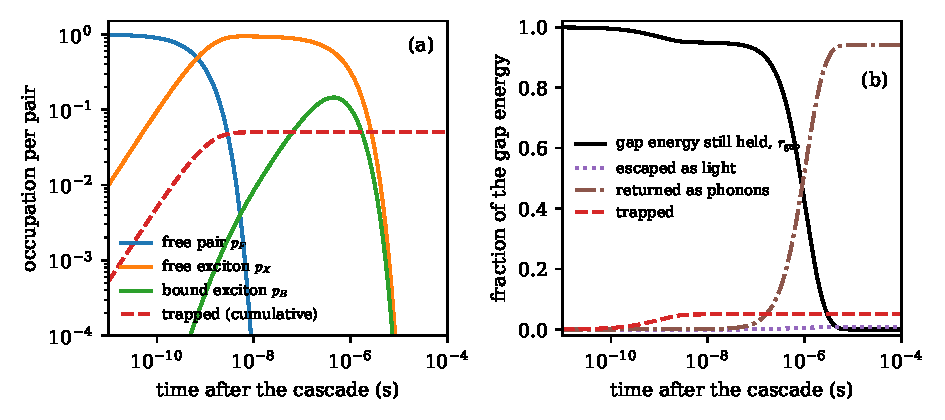
\includegraphics[width=\linewidth]{figures/ch18/fig18_4.pdf}
  \caption{End-of-cascade populations of one electron--hole pair in silicon at \SI{50}{mK}, from the rate equations \cref{eq:18.5-rates} with one species of neutral impurity. (a)~Occupations of the free pair, the free exciton and the bound exciton, and the cumulative trapped fraction, against the time after the cascade. (b)~Fraction of the gap energy still held by pairs and excitons, $r_{\mathrm{gap}}$ of \cref{eq:18.5-rgap}, and the cumulative fractions returned as phonons, escaped as light and trapped. Rates: bound-exciton Auger decay \SI{250}{ns}, inside the measured 200 to \SI{300}{ns} of the phosphorus donor~\cite{lo2015hybrid}, without light. Illustrative, since none is measured at \SI{50}{mK}: binding of the pair \SI{1}{ns}, trapping $\varGamma_{FT} = 0.053\varGamma_{FX}$, binding of the free exciton to impurities \SI{1}{\micro s}, free-exciton decay \SI{10}{\micro s} with luminescent fraction 0.1. Asymptotic split \cref{eq:18.5-split}: 0.050 trapped, 0.009 light, 0.941 phonons.}
  \label{fig:18-end}
\end{figure}

\subsection{Unknown rates and unsized truncations}\label{sec:18.5-open}

The rates of \cref{eq:18.5-rates,eq:18.5-traps} are the main unknowns of this section. In silicon and germanium at 10 to \SI{50}{mK}, no measurement or calculation gives the rate at which a cold pair binds, or the coefficient of binding between carriers of different pairs. The same holds for the capture cross-sections of cold and drifting carriers on charged and neutral centers, as functions of carrier energy, temperature and field, and for the cross-sections for binding of excitons to each impurity species. Also unknown are the decay rate and luminescent fraction of the free exciton, the luminescent fractions of the bound excitons, and the coefficients of exciton--exciton annihilation and of Auger recombination that govern dense tracks. The thresholds at which dense pairs condense into electron--hole droplets, the degenerate electron--hole liquid of germanium and silicon, are open as well at millikelvin temperatures. What is known are the binding energies, \SI{14.7}{meV} in silicon and a few meV in germanium, and the Auger lifetimes of bound excitons at liquid-helium temperature, a property of the complex in its ground state that should carry over to lower temperatures. The excitons themselves cool by emitting acoustic phonons, slowly at these temperatures, so their temperature need not be that of the lattice, and rates measured at a few kelvin cannot simply be transferred.

The cascade hands over less than these equations need. No material has a computed capture probability $f(x)$ as a function of the terminal energy of a carrier, nor the distribution of terminal energies on which \cref{eq:18.5-thingen} averages it. Nor is the separation of the pairs at the end of the cascade, which decides through \cref{eq:18.5-rfield} whether a field prevents binding. In the ionic crystals, where the cascade quantum may be a bound pair, the exciton binding energies and the binding to impurities are open as well.

Two approximations of the cascade itself remain unsized. A constant factor of 0.8 on the impact-ionization rate, the quasiparticle residue left out of \cref{eq:18.1-ii}, changes $\varepsilon_{\mathrm{eh}}$ by about \SI{3}{\percent}, and calibrating on the measured pair energy removes it. A factor that varies with the carrier energy between threshold and about \SI{10}{eV}, as the residue and the carrier--electron exchange may, changes $F_{\mathrm{eh}}$, and its size is not known. For the energy-only reduction, the probability that a carrier keeps its momentum between two events that change its energy is estimated to be below about 0.1 within \SI{1}{eV} of threshold, where intervalley scattering dominates, and to reach one half above 3 to \SI{5}{eV} in silicon. A full-band cascade finds the resulting memory negligible, but only within the deformation-potential model of the phonons (\cref{sec:18.1-reductions}); with first-principles couplings, which do not redraw the crystal momentum at every emission, neither this probability nor the spread over the iso-energy surface that it multiplies has been computed.

\section*{Summary}

A hot carrier in a semiconductor is a projectile of the master formula (\cref{sec:18.1}). Its impact ionization is the rate \cref{eq:18.1-ii}, whose kernel is the screened interaction, and phonon emission is the same formula with the electron--phonon vertex; momentum conservation puts the impact-ionization threshold at $\theta_{\mathrm{ii}}\Eg$, with $\theta_{\mathrm{ii}} = 3/2$ for equal masses. The cascade is a branching process whose statistics follow from one generating functional and its backward equation \cref{eq:18.1-backward}, and the energy identity \cref{eq:18.1-energy} ties every fluctuation of the pair number to a fluctuation of the heat. The cascade must be seeded class by class: at \SI{10}{eV} an equal split of the energy between electron and hole yields 2.985 pairs on average, and a uniform distribution of splits with the same mean split yields 2.691.

The mean energy per pair and the Fano factor are the first two moments of that generating functional (\cref{sec:18.2}). $F_{\mathrm{eh}}$ is the variance of the heat per pair in units of $\Eg^2$; in silicon its three terms add to $0.092 + 0.290 - 0.268 = 0.114$. Below about $15\Eg$ the yield rises in steps of one pair, so that a search at a few pairs needs the whole pair-number distribution.

At \SI{5}{eV} in silicon a dark-matter kick at $q_0$ puts two pairs in \SI{17}{\percent} of events, where the step model puts two in every event (\cref{sec:18.3}). The step model and fixed splits of the energy fail between 4.4 and \SI{13}{eV}, where the split decides the count. Against a full-band cascade with no fitted constant, the step model overcounts the two-pair bin about tenfold, and at least sixfold anywhere in the envelope of the full-band variants.

With its one constant fixed by the measured pair energy of silicon, the cascade yields $F_{\mathrm{eh}} = 0.114$ against the measured $0.119 \pm 0.002$ (\cref{sec:18.4}). The full-band cascade gives $\varepsilon_{\mathrm{eh}} = \SI{4.15}{eV}$ $[3.95, 4.73]$ against the measured \SI{3.749}{eV}. The calibrated cascade reduces over its parameter range to the observed linear law $\varepsilon_{\mathrm{eh}} \approx 1.61\Eg + k_2$. Against the seven crystals besides silicon with a measured pair energy, the residuals of the calibrated cascade run from $-\SI{19.8}{\percent}$ to $+\SI{7.0}{\percent}$ (root mean square \SI{10.5}{\percent}). The crystals with a measured pair energy, silicon included, span the validated range of the calibrated cascade, and the halides, fluorides, lead salts and InSb lie outside that range.

Below the impact-ionization threshold the pair number can still change (\cref{sec:18.5}). A capture probability $f_{\mathrm{cap}}$ shared by all electrons turns $\varepsilon_{\mathrm{eh}}$ into $\varepsilon_{\mathrm{eh}}/(1 - f_{\mathrm{cap}})$ and $F_{\mathrm{eh}}$ into $(1 - f_{\mathrm{cap}})F_{\mathrm{eh}} + f_{\mathrm{cap}}$, and a loss of \SI{0.54}{\percent} would account for the difference between the cascade value and the measured Fano factor of silicon. Excitons change neither the pair number nor its moments; they return their binding energy as heat, and an exciton that is never split thins the measured charge, \cref{eq:18.5-Fmeas}. Almost none of the rates of capture, exciton binding and trapping is known at millikelvin temperatures.

\printbibliography[heading=subbibliography]
